\documentclass[11pt]{book}

%\usepackage{jcappub}
\usepackage{style}

\usepackage[utf8]{inputenc}   % Allows UTF-8 character encoding
\usepackage{amsmath}          % For advanced math typesetting
\usepackage{amssymb}          % Additional math symbols
\usepackage{graphicx}         % For including images
\usepackage{hyperref}         % For hyperlinks in the document
\usepackage{geometry}         % For setting up page geometry
\usepackage{siunitx}          % For consistent typesetting of units
\usepackage{float}            % To control float positioning (e.g., figures/tables)
\usepackage{enumitem}         % Better control over list formatting
\usepackage{tocloft}
\usepackage{tikz}
\usepackage{tikz-3dplot}
\usetikzlibrary{shapes.geometric, arrows, backgrounds}
\usepackage{empheq}
\usepackage{booktabs}
\usepackage{multirow} % needed for merging cells vertically
\usepackage{booktabs}
\usepackage{xcolor}


\usepackage{listings}
\usepackage{xcolor}
\usepackage{pgfmath}
\newcommand{\greenfactor}[1]{%
    \pgfmathsetmacro{\value}{min(100,round(100*(#1-1)))}%
    \textcolor{green!80!black!\value!black}{#1}%
}


\usepackage[backend=bibtex, sorting=none]{biblatex}
\addbibresource{sources_updated.bib}

% some custom commands that should've already been in latex by default
\DeclareRobustCommand{\d}{\ifmmode\text{d}\else d\fi}
\DeclareRobustCommand{\Cov}{\ifmmode\text{Cov}\else d\fi}
\DeclareRobustCommand{\PSF}{\ifmmode\text{PSF}\else d\fi}
\DeclareRobustCommand{\CMB}{\ifmmode\text{CMB}\else d\fi}
\DeclareRobustCommand{\gal}{\ifmmode\text{gal}\else d\fi}
\DeclareRobustCommand{\obs}{\ifmmode\text{obs}\else d\fi}
\DeclareRobustCommand{\intr}{\ifmmode\text{intr.}\else d\fi}
\DeclareRobustCommand{\tr}{\ifmmode\text{tr}\else d\fi}
\DeclareRobustCommand{\tf}{\ifmmode\text{tf}\else d\fi}

\newcommand{\Rstar}{R_\ast}
\newcommand{\deltaD}{\delta_{\mathrm D}}

\newcommand{\br}[1]{\ensuremath{\left( #1 \right)}}
\newcommand{\sbr}[1]{\ensuremath{\left[ #1 \right]}}

\newcommand{\reviewnote}[1]{\textcolor{red}{[\textbf{Review:} #1]}}

\setlength{\cftbeforesecskip}{5pt}

% Additional customizations (optional)
\setlength{\parindent}{0pt}   % No paragraph indentation
\setlength{\parskip}{1em}     % Add space between paragraphs
\title{Galaxy B Modes}

\author{Jonas Frugte}


\begin{document}

\maketitle

\setcounter{tocdepth}{1}
\tableofcontents

\chapter{Introduction and Motivation}
TODO

\chapter{Bias, Effective Field Theory (EFT), Intrinsic Alignment}
\section{Halo Bias and EFT}
In this section we introduce the much more established field of galaxy bias and an EFT of galaxy bias. This will directly translate to the EFT used in section \ref{sec:galaxyintrinsicalignment}. We consider a $\Lambda$CDM universe with a perturbed FLRW metric unless stated otherwise.

\subsection{What is bias}
Say we look at a the universe at redshift $z$. Given a perturbation to the matter density $\delta(\mathbf x, z)$ we would like to know the perturbation to the density of some other tracer. In this section we will consider the relative number overdensity of dark matter halos, $\delta_h$, but the results are applicable to any tracer in general, notably to galaxy number density. We then model the relation between these two as
\begin{equation}
    \delta_h(\mathbf x, z) = \sum_{\mathcal O} b_{\mathcal O}(z) \mathcal O(\delta)(\mathbf x, z),
\end{equation}
where we sum over some set of operators $\{\mathcal O\}$ that map $\delta$ to a new function of position and time and the $b_{\mathcal O}$ are the BPs. Crucially, they only depend on z and not on $\mathbf x$. 4 questions arise naturally from this model:
\begin{enumerate}
    \item What is the motivation to use this model? Why is this expected to be accurate up to a (reasonably small) scale cutoff with the right choice of operators and values of BPs?
    \item How can we choose a set of operators that is "complete"? I.e. that the model is correct in the sense of the previous question.
    \item How do the bias parameters evolves over time?
    \item How do we determine bias parameters? Both theoretically and empiricially given a dataset from a real life survey or a simulation.
\end{enumerate}
The rest of this section will be devoted to summarizing the answers to these questions.


\subsection{Relating bias parameters from different times}
We consider a simple case where a population of galaxies instantly formed at some time $\tau_*$. This is sufficient because the evolution equations we obtain will then work as a ``Green's function'' for the evolution equations of bias parameters in general. We simply integrate over the time evolved bias parameters weighted by the rate of galaxy formation at the integrand time.

We assume that whatever tracer we consider moves with the fluid. This immediately gives the continuity equation:
\begin{equation}
    \frac{D}{D\tau}\delta_g = -\theta(1+\delta_g),
    \label{eq:conteqtracer}
\end{equation}
where
\begin{equation}
    \frac{D}{D\tau} = \frac{\partial}{\partial \tau} + v^i\frac{\partial}{\partial x^i}
\end{equation}
is the convective time derivative, $v^i$ is the peculiar velocity of the cosmic matter fluid, and $\theta=\partial_i v^i$ is the velocity divergence. % TODO: mention something about assuming no velocity bias?
To evolve $\delta_g$ we also need evolution equations for $\delta$ and $v^i$. They are given by the continuity equation (again)
\begin{equation}
    \frac{D}{D\tau}\delta = -\theta(1+\delta),
    \label{eq:conteq}
\end{equation}
and the Euler equation,
\begin{equation}
    \frac{D}{D\tau}\theta = -\mathcal H \theta - (\partial^iv^j)^2 - \frac{3}{2}\Omega_m\mathcal H^2\delta.
\end{equation}
% TODO: say something about the different ways of solving these eqs?

We proceed by dividing equations \ref{eq:conteq} and \ref{eq:conteqtracer} by $1+\delta$ and $1+\delta_g$, respectively to get
\begin{equation}
    \frac{1}{1+\delta_g}\frac{D}{D\tau}\delta_g = \frac{1}{1+\delta}\frac{D}{D\tau}\delta.
\end{equation}
This can be solved by switching to Lagrangian coordinates to get
\begin{equation}
    \ln (1+\delta_g(\mathbf x (\tau), \tau)) = \ln (1+\delta(\mathbf x (\tau), \tau)) + \ln (\frac{1+\delta_g(\mathbf x (\tau), \tau)}{1+\delta(\mathbf x(\tau), \tau)}), \quad \tau>\tau_*,
\end{equation}
which can be written more simply as
\begin{equation}
    1+\delta_g|_\tau = \frac{1+\delta|_\tau}{1+\delta|_{\tau_*}}(1+\delta_g|_{\tau_*}).
\end{equation}
This equation can be made usefull by expanding order by order. Up to second order we get
\begin{gather}
    1+\delta_g^{(1)}(\mathbf x, \tau) + \delta_g^{(2)}(\mathbf x, \tau) = 1+\delta^{(1)}-\delta^{(1)}_* + \delta_{g*}^{(1)}+\delta^{(2)}-\delta{(2)}_*+\delta_{g*}^{(2)}+[\delta_*^{(1)}]^2-\delta^{(1)}\delta^{(1)}_*+\sbr{\delta^{(1)}-\delta_*^{(1)}}\delta_{g*}^{(1)}.
\end{gather}
Now, the difference between $\mathbf x$ and $\mathbf x_*$ is first order in perturbations as well. We can Taylor expand around $\mathbf x$ and use that the displacement, $\mathbf x - \mathbf x_*$ evolves according to the growth factor $D$ to get
\begin{align}
    \delta^{(1)}_g(x,\tau) &= \left( 1 + \frac{D_*}{D}\,[b_1^* - 1] \right) 
       \delta^{(1)}(x,\tau) + \varepsilon^* \\[6pt]
    \delta^{(2)}_g(x,\tau) &= \left\{ 1 + [b_1^* - 1] \left(\frac{D_*}{D}\right)^2 \right\}\delta^{(2)} 
       + \left\{ \frac{D_*}{D}[b_1^* - 1] - \left(\frac{D_*}{D}\right)^2[b_1^* - 1] 
       + \tfrac{1}{2} b_2^* \left(\frac{D_*}{D}\right)^2 \right\} [\delta^{(1)}]^2 \\[6pt]
       &\quad + b_K^{*2}\left(\frac{D_*}{D}\right)^2 [K^{(1)}_{ij}]^2
       + \left(\frac{D_*}{D} - 1\right)\frac{D_*}{D}[b_1^* - 1]\,s_{(1)}^i \partial_i \delta^{(1)}
       - \left(\frac{D_*}{D} - 1\right)\varepsilon^* \delta^{(1)} \\[6pt]
       &\quad + \left(\frac{D_*}{D} - 1\right) s_{(1)}^i \partial_i \varepsilon^* \,.
\end{align}
Here, $\varepsilon$ is a stochastic parameter added in and $s^i=x^i-x^i_*$ is the displacement. One can then extract the bias parameters at current time (Eularian time) by comparing to the bias expansion at Eularian time and matching terms to get
\begin{align}
    b_1^E &= 1 + \frac{D_*}{D}(b^*_1-1) \\
    b_2^E &= b_2^* \br{\frac{D_*}{D}}^2 + \frac{8}{21}\br{1-\frac{D_*}{D}}(b_1^E-1) \\
    b_{K^2}^E &= b^*_{K^2} \br{\frac{D_*}{D}}^2 - \frac{2}{7}\br{1-\frac{D_*}{D}}(b_1^E-1)
\end{align}
Clearly this can be easily generalized to any order.


\subsection{EFT of bias parameters}
%TODO: explain lagrangian and eularian space
Main ref: \cite{Desjacques_2018}
We would like to find a "basis" of bias parameters up to a given order in perturbation theory. We will assume that (1) gravitation is described by general relativity, (2) that we can neglect the impact of massive neutrinos and dark energy perturbations, (3) that initial conditions are Gaussian and adiabatic.

\emph{We will assume that the only quantities relevant for the formation of galaxies are local on some scale} $R_*$ (which is much larger than the size of a galaxy / whatever tracer we are considering). According to the equivalence principle, the only effects that can be measured by a freely falling observer (i.e. forming galaxy) is the second derivatives of the gravitational potential, $\partial_i \partial_j \Phi$. Higher derivatives will be higher order contributions, because each derivative on a scale of $R_*$ contributes a factor of $k/R_*$, which for large enough scales will be much smaller than one.

Now, the galaxy density, $\delta_g$ %TODO: give proper def of delta_g
will in a very general sense depend on the history of $\partial_i \partial_j \Phi$ along the fluid trajectory. In other words:
\begin{equation}
    \partial_g(\mathbf x, \tau) \supset \int^\tau d\tau'f_{\mathcal O }(\tau, \tau') \mathcal O (\mathbf x_{fl}(\tau'), \tau'),
\end{equation}
where $f_O$ is some kernel that we don't need to bother defining. %TODO: is there anything more we can say about it?
We can then Taylor expand to get
\begin{equation}
    \partial_g(\mathbf x, \tau) \supset \sbr{\int^\tau d\tau'f_{\mathcal O }(\tau, \tau')} \mathcal O (\mathbf x_{fl}(\tau), \tau) + \sbr{\int^\tau d\tau' (\tau'-\tau) f_{\mathcal O }(\tau, \tau')} \frac{D}{D\tau}\mathcal O (\mathbf x_{fl}(\tau), \tau) + \cdots,
\end{equation}
where $D/D\tau$ is the convective derivative along the fluid flow. %tTODO: give mathematical definition 
In order to define a basis we thus also have to include time derivatives $D/D\tau$ of the second derivatives of the potential. It now seems like we would need an infinite set of operators to form a basis. This can be avoided by noticing at finite order in perturbation theory, only a finite amount of these operators are linearly independent of one another.

In order to show the above statement, we will first switch to Lagrangian coordinates $\mathbf q = \mathbf x_{fl}(\tau=0)$ where the convective time derivative simplifies to $\partial/\partial \tau$. We also assume that the $n$-th order growth factor is given by the linear growth factor to the $n$-th power. This is only strictly valid for an EdS (flat matter dominated universe) but is still very accurate for other cosmologies such as $\Lambda$ CDM. % TODO: when are you even allowed to use a growth factor? check this
Consider some operator in the basis, $O_L(\mathbf q, \tau)$ which has contributions at various orders, $O_L^i(\mathbf q, \tau)$, then
\begin{equation}
    \br{\frac{D}{D\tau}}^n O_L(\mathbf q, \tau)|^{(n)} = \br{\frac{\partial}{\partial\tau}}^n O_L(\mathbf q, \tau)|^{(n)} = \sum_{i = 1}^n \br{\frac{d^n}{d\tau^n}D^i(\tau)}O^{i}_{L}(\mathbf q, \tau_0).
\end{equation}

Next, although higher order contributions start being linearly dependent on the lower order contributions after some order, as shown above, it is worth noting that these higher order contributions are in general no longer local in $\partial_i\partial_j \phi$. This is immediately obvious if we notice that the convective time derivative contains a spatial derivative that generates higher order ($k/R_*$) terms. It turns out that, due to symmetry requirements, we only need to consider $\partial_i \partial_j / \nabla ^2$ acting on powers of $\partial_k \partial_l \Phi$ in order to get all the new terms created by the extra spatial derivatives. % TODO: find a proper proof of this, "Large Scale Galaxy Bias" just kind of brushes over this imo, can check out McDonald & Roy (2009)
% TODO: okay so apparently this basis is only for terms local in spatial derivatives, so we do actually get extra terms given by spatial derivatives.

Constructing a \emph{local} Eularian basis out of $\partial_i\partial_j\Phi(\mathbf x, \tau)$ and its convective time derivatives can be done explicitly as first shown in \cite{Mirbabayi_2015}. First define
\begin{equation}
    \Pi^{[1]}_{ij}(\mathbf x, \tau) = \frac{2}{3\Omega_m\mathcal H^2}\partial_i\partial_j\Phi(\mathbf x, \tau) = K_{ij}(\mathbf x, \tau) + \frac{1}{3}\delta_{ij}\delta(\mathbf x, \tau)
\end{equation}
and
\begin{equation}
    \Pi^{[n]}_{ij} = \frac{1}{(n-1)!}\sbr{ \frac{1}{\mathcal H f}\frac{D}{D\tau} \Pi^{[n-1]}_{ij} - (n-1)\Pi^{[n-1]}_{ij}},
\end{equation}
as given by ref. \cite{Mirbabayi_2015}. Then take into account that $\tr \Pi^{[n]}$ can be written in terms of lower order operators through the Eularian fluid equations. % TODO: introduce/discuss them very briefly

To get all terms at order $n$, we then write products of $\Pi^{[k]}$ where $k<n$ and the total order adds up to $n$ or less and take traces of the different possible combinations of each product. %TODO: describe this better somehow

Thusfar we have only considered an expansion local in the second derivatives of the gravitational potential. Higher order derivatives can and should also be considered. Assume that all relevant nonlocal effects are limited to some scale, the "scale of nonlocality" $R_*$. Following the reasoning in \cite{Schmidt2013_clustering}, nonlocal contributions to the tracer number density at $\mathbf x$ will come from terms at $\mathbf x + \mathbf y$, where $y \sim R_*$. Take, for example, $\delta(\mathbf x + \mathbf y)$. Through a Taylor expansion at $\mathbf x$ we thus find that this contribution can be written as
$$
b_{\delta(\mathbf x + \mathbf y)}\delta(\mathbf x+\mathbf y) = b_{\delta(\mathbf x + \mathbf y)}(\delta(\mathbf x) + \mathbf y \cdot\vec \nabla \delta(\mathbf x) + y^2\nabla^2\delta(\mathbf x) + \cdots).
$$
Terms with an odd order of derivatives will not contribute due to isotropy. On the other hand, $y^2\nabla^2\sim R_*^2 k^2$ in Fourier space. We thus see that for scales much larger than the non-locality scale (the regime in which we expect biasing to work anyway), higher derivative terms are surpressed through the factor $R_*^{2n}k^{2n}\ll 1$, where $n$ is the order of the derivative. Note that we assume that the BP's themselves are not much larger than 1, and if we find that that is not the case then there's a sign that our perturbative expansion has stopped working for the scales considered. When aiming to find a full basis for our expansion up to some order, we thus need to consider the tracer in question to know up to which order in derivatives and perturbation theory to work. % TODO: check this? should I use "perturbation theory" here?

% Some math I did regarding this stuff:
% \begin{gather}
%     \lim_{R \rightarrow 0}\frac{1}{R}\sbr{f_{R_*}(x+R) - f_{R_*}(x)} \\
%     = \lim_{R \rightarrow 0} \frac{1}{2RR_*}\sbr{\int_{x+R-R_*}^{x+R+R_*}f(y)\d y - \int_{x-R_*}^{x+R_*}f(y)\d y} \\
%     = \lim_{R \rightarrow 0} \frac{1}{2RR_*}\sbr{\int_{x+R_*}^{x+R+R_*}f(y)\d y - \int_{x-R_*}^{x+R-R_*}f(y)\d y} \\
%     = \lim_{R\rightarrow 0} \frac{R}{2RR_*}\sbr{f(\xi_+) - f(\xi_-)} \quad \text{(Mean Value Thm)}\\
%     =\frac{f(x+R_*) - f(x-R_*)}{2R_*} \\
%     \xrightarrow{FT} \frac{f(k)}{2R_*}\br{e^{ikR_*} - e^{-ikR_*}} \\
%     = \frac{f(k)}{R_*}i\sin \br{kR_*} \\
%     \begin{cases}
%         \approx ikf(k) & k R_* \ll 1\\
%         \sim f(k)/R_* & \text{else} 
%     \end{cases}
% \end{gather}

\section{Spin-2 Fields and Their Projections}
It is well known how to construct powerspectra from scalar quantities. Constructing them for a spin-2 field requires more care. In particular, we would like to find a way to define powerspectra that is independent of the orientation of the observer.

We model galaxies in 3D space as ellipsoids where we do not care about the overal size. This means they can be described according to the $3 \times 3$ symmetric trace-free tensor $Q_{ij}$ given by
\begin{equation}
    Q_{ij} = \tf\br{\frac{\int \d^3 x \rho(\mathbf x) x^i x^j}{\int\d^3 x \rho(\mathbf x)}},
\end{equation}
where we assume for simplicity that the galaxy's center of mass is at $x^i=0$ and $\tf (\cdot)$ means taking the trace free part. The trace corresponds to the overal size of the galaxy and is not of interest to us. This corresponds roughly to $g_{ij}$ from \cite{bakx2023effectivefieldtheoryintrinsic}.
$Q_{ij}$ at some point can transform under SO(3). Specifically, it transforms under the spin-2 representation, which can immediately be seen because $Q_{ij}$ is a 5 dimensional vector space and there is only one irreducible representation of SO(3) of dimension $2\ell + 1$, with in this case $\ell = 2$. This is the classification theorem. %TODO: give citation
Alternatively, it is clear that under a SO(3) rotation given by $R$, we get $Q_{ij} \rightarrow R_{ia}R_{jb}Q_{ab}$. One can compare this to the spin-2 representation of SO(3) to see that they are the same. %TODO: find source?

We observe shapes as projected onto the sky. If we take $\mathbf n$ as our line of sight with associated projection matrix $P^{ij}$, then
\begin{gather}
    \gamma_{ij} := \tf_P\br{P^{ik}P^{jl}g_{kl}(\mathbf x, z)}\\
                = \frac{1}{2}\br{P^{ik}P^{jl} + P^{il}P^{jk} - P^{ij}P^{kl}}g_{kl}(\mathbf x, z)\\
                =: P^{ijkl}g_{kl}(\mathbf x, z).
\end{gather}
In the last line we simply define $P^{ijkl}$ as the combination of $P^{ij}$ from the line above. Going from line 1 to line 2 follows by using that in the projected space, the metric is $P^{ij}$ instead of $\delta^{ij}$ and the trace of an arbitrary tensor $M_{ij}$ thus becomes $P^{ij}M_{ij}$. % TODO: explain better why this is, because I'm not 100 percent convinced of this myself

$\gamma_{ij}$ is again symmetric, trace-free, and transforms like a spin-2 representation, now of SO(2).

\subsection{Spherical tensor decomposition}
Going back to the non-projected $Q_{ij}$, it's clear that this tensor is defined at each point in space, $\mathbf x$. Now look at the Fourier transform, $Q_{ij}(\mathbf k)$. For a mode in a given direction, $\hat{\mathbf k}$, we can decompose $Q_{ij}(\mathbf k)$ through the spherical tensors $(Y_2^{(m)})(\hat{\mathbf k})_{ij}$, with $m=-2, -1, 0, 1, 2$ denoting the helicity. %TODO: add source
We get
\begin{align}
    (Y_2^{(0)})(\hat{\mathbf k})_{ij} &= \sqrt{3/2}(\hat{\mathbf k}_i\hat{\mathbf k}_j - \frac{1}{3}\delta_{ij})\\
    (Y_2^{(\pm 1)})(\hat{\mathbf k})_{ij} &= \sqrt{1/2}(\hat{\mathbf k}_i\mathbf e_j^\pm + \hat{\mathbf k}_j\mathbf e_i^\pm)\\
    (Y_2^{(\pm 2)})(\hat{\mathbf k})_{ij} &= \mathbf e_i^\pm \mathbf e_j^\pm
\end{align}
with $e^{\pm}=...$%TODO
and $i,j=1,2,3$. The unit vectors $e_1$ and $e_2$ are defined by $...$ %TODO
For a rotation around $\hat{\mathbf k}$ by an angle $\phi$ the spherical tensors transform as
$$
(Y_2^{(m)})(\hat{\mathbf k})_{ij} \rightarrow e^{im\phi}(Y_2^{(m)})(\hat{\mathbf k})_{ij}.
$$
These spherical tensors have a number of other usefull properties which we will not get into right now. 

\subsection{Defining Power Spectra}
We can now define the powerspectrum as a $3 \times 3 \times 3 \times 3$ tensor given by
\begin{equation}
    \langle Q_{ij}(\mathbf k)Q_{ij}(\mathbf k') \rangle = (2 \pi)^3\delta^D(\mathbf k + \mathbf k')P_{ijkl}^{QQ}(\mathbf k).
\end{equation}
This definition is the most obvious, however because $Q_{ij}$ transforms as a tensor under rotations, it leaves $P_{ijkl}^{QQ}(\mathbf k)$ dependent on the direction of $\mathbf k$. We can instead work with the decomposition of $Q_{ij}$ in the spherical tensors:
\begin{equation}
    Q_{ij}(\mathbf k) = \frac{1}{3}\delta_{ij}Q_0^0(\mathbf k) + \sum_{m=-2}^2Q_2^m(\mathbf k)Y_{ij}^{(m)}(\hat{\mathbf k}),
\end{equation}
where we now allow $Q_{ij}$ to also have a trace / scalar component $Q_0^0$. % TODO: this transition is a bit abrupt, should make this the case from the start
We can then define the following powerspectra:
\begin{equation}
    \langle Q_l^{(m)}(\mathbf k)Q_{l'}^{(m')}(\mathbf k')\rangle = (2\pi)^3\delta_{mm'}\delta^D(\mathbf k + \mathbf k')P^{(m)}_{ll'}(k).
\end{equation}
When the powerspectra are defined in this way, they are scalars. There are 7 independent spectra, however we also have by the properties of the spherical tensors that
\begin{equation}
    P_{ll'}^{(m)}(k)^*=P_{ll'}^{(-m)}(k).
\end{equation}
If we also enfore invariance under parity transformations, then we find that the powerspectra are real and thus that
\begin{equation}
    P^{(m)}_{ll'}(k)=P^{(-m)}_{ll'}(k).
\end{equation}
This reduces the amount of independent spectra to 5. % Don't you also get this if there's no parity invariance? this part is a bit sketch ngl

\subsection{Noise power spectra}
\label{sec:noisepowerspectragalaxyIA}
In accordance with the previous subsection, there are 3 power spectra due to stochastic / noise terms in the EFT of galaxy IA. They come from combinations of scalar / galaxy size noise and spin-2 / symmetric traceless tensor / galaxy shear noise.
\begin{align}
    \langle \epsilon(\mathbf k)\epsilon(\mathbf k') \rangle' &= P^s_\epsilon(k), \\
    \langle \epsilon_{ij}(\mathbf k)\epsilon(\mathbf k') \rangle' &= (\mathbf k_i \mathbf k_j - \frac{1}{3} \delta_{ij}k^2)P^{gs}_\epsilon(k), \\
    \langle \epsilon_{ij}(\mathbf k)\epsilon_{kl}(\mathbf k') \rangle' &= (\delta_{ik}\delta_{jl}+\delta_{il}\delta_{jl}-\frac{2}{3}\delta_{ij}\delta_{kl})P^g_\epsilon(k) .
\end{align}
In all three cases $P_{\epsilon}^{\cdots}(k) = c^{\cdots} + \mathcal O(R^2k^2)$. The forms of the spectra are again constructed to satisfy transformation properties, symmetry, and tracelessness. For the scalar-scalar and tensor-tensor spectra the above equations correspond to white noise with some corrections terms that only become significant if the scales we are looking at ($1/k$) become comparable to the scale of nonlocality of galaxy formation ($R$). For the tensor-scalar correlation there is no `white noise' (or term independent of $k$). To see why, consider what would happen if $P^{gs}_\epsilon(k)$ would have a $k^{-2}$ term.
\begin{equation}
    \langle \epsilon_{ij}(\mathbf k)\epsilon(\mathbf k') \rangle' \supset \br{ \frac{\mathbf k_i\mathbf k_j}{k^2} - \frac{1}{3}\delta_{ij}} \xrightarrow{\mathcal F^{-1}}\propto (\partial_i\partial_j\nabla^{-2} - \frac{1}{3}\delta_{ij})\delta^{3}(\mathbf x) \supset \propto \frac{1}{x^3}.
\end{equation}
This means that we have nonlocality on scales larger than the nonlocality scale of galaxy IA, which shouldn't be possible.

\subsection{$E$ and $B$ modes of spin-2 field}
A field of spin-2 tensors on the sphere can also be decomposed into $E$ and $B$ modes. $E$ modes correspond to a divergence like field while $B$ modes create a curl like field. Their key property is that, under a parity transformation, $B$ modes change sign while $E$ modes stay the same.

To calculate these modes, first decompose the spin-2 field into spin-2 spherical harmonics. We are now working on the sphere, so the spin-2 tensors, i.e. the shear, is given by a complex number $_{\pm 2} X(\hat {\mathbf n})$. It transforms under a local rotation by an angle $\alpha$ as 
\begin{equation}
    _{\pm 2}X(\hat{\mathbf n}) \rightarrow e^{\mp 2i\psi} \,_{\pm 2}X(\hat{\mathbf n}).
\end{equation}

The decomposition to spin 2 spherical harmonics is given through the usual inner product. We thus obtain spin $a_{\pm 2,lm}$'s. We define the $E$ and $B$ modes through their spherical harmonic coefficients as
\begin{gather}
    E_{lm} = -\frac{1}{2}\br{a_{2,lm} + a_{-2,lm}}\\
    B_{lm} = \frac{i}{2}\br{a_{2,lm} - a_{-2,lm}}.
\end{gather}


\section{EFT of Galaxy IA}
\label{sec:galaxyintrinsicalignment}
\subsection{Local Deterministic Terms}
To get the EFT of galaxy IA, we use $\Pi^{[n]}$ again (equation ... %TODO: ref
) but instead of making scalar combinations we make symmetric trace free combinations of the form
\begin{equation}
    Q_{ij}(\mathbf x, \eta) = \sum_{\mathcal O}b_{\mathcal O}(\eta)\mathcal O_{ij}(\mathbf x, \eta).
    \label{eq:shapebiasdeterministic}
\end{equation}
Up to order 3 we get the following local deterministic contributions \cite{Vlah_2020}:
\begin{itemize}
    \item[] 1st order: $\tf[\Pi^{[1]}]_{ij}$ 
    \item[] 2nd order: $\tf[\Pi^{[2]}]_{ij}$, $\tf[(\Pi^{[1]})^{2}]_{ij}$, $\tf[\Pi^{[1]}]_{ij}\tr \Pi^{[1]}$
    \item[] 3rd order: $\tf[\Pi^{[3]}]_{ij}$, $\tf[(\Pi^{[1]}\Pi^{[2]})]_{ij}$, $\tf[\Pi^{[2]}]_{ij}\tr \Pi^{[1]}$, $\tf[(\Pi^{[1]})^{3}]_{ij}$, $\tf[(\Pi^{[1]})^{2}]_{ij}\tr \Pi^{[1]}$, $\tf[\Pi^{[1]}]_{ij}(\tr \Pi^{[1]})^2$, $\tf[\Pi^{[1]}]_{ij}\tr ((\Pi^{[1]})^2)$
\end{itemize}
We do not need to include factors of the form $\tr(\Pi^{[n]})$ for $n>1$. This was first argued and shown explicitly up to $n=3$ in \cite{Mirbabayi_2015}. In short, we do not need to include this factor because by using the continuity, Euler, and Poisson equations one can write $\tr(\Pi^{[n]})$ as other terms included elsewhere in the bias expansion.
\subsection{Non-local deterministic Terms}
As explained in subsection ... %TODO
we should also consider non-local terms, which are surpressed by orders of $(R_*k)^2$ (or $(R_*\nabla)^2$ in real space). At one loop order (when calculating power spectra) it suffices to go up to first order in nonlocality \cite{Mirbabayi_2015}, in which case the only new term in our basis is
$$
R^2_*\nabla^2\tf(\Pi^[1])_{ij}.
$$
The ratio between non-local and SPT contributions to a power spectrum can be calculated as ... \\
TODO here: explain this, justify why only one order is needed, give indication to what order of SPT this corresponds

\subsection{Stochastic Terms}
Due to our lack of knowledge about small scale modes, we get stochastic terms in our basis. In analogy to stochastic contributions to galaxy bias \cite{Desjacques_2018}, we generalize equation \ref{eq:shapebiasdeterministic} to \cite{Vlah_2020}
\begin{equation}
    g_{ij}(\mathbf x, \tau) = \sum_{O}\sbr{b^{(g)}_{O}(\tau) + \epsilon_O(\mathbf x, \tau)} O_{ij}(\mathbf x, \tau) + \epsilon_{ij}^O(\mathbf x, \tau) O(\mathbf x, \tau) + \epsilon_{ij}(\mathbf x, \tau).
\end{equation}
The $\epsilon$ fields are uncorrelated with the $O_{ij}$, have vanishing expectation value and are completely described by their one-point distribution, i.e. $\langle \epsilon_O(\mathbf x) \epsilon_{O'}(\mathbf x') \rangle \propto \delta(\mathbf x - \mathbf x')$. %TODO: is this correct? what about up to order R_*^2k^2?
Each $\epsilon_{ij}$ respects the same symmetries as $g_{ij}$. The $O$'s are the scalar terms that one would consider in e.g. a galaxy bias EFT. $\epsilon_{ij}$ describes the leading order shape noise (when projected to the sky), see also subsection ... .
In general, the stochastic contributions up to third order are given by 
\begin{itemize}
    \item[] 1st order: $\epsilon_{ij}$,
    \item[] 2nd order: $\epsilon_{ij}^\delta\tr\sbr{\Pi^[1]}$, $\epsilon_{\Pi^{[1]}}\tf\sbr{\pi^{[1]}}_{ij}$,
    \item[] 3rd order: $\epsilon_{ij}^{\delta^2}\br{\tr\sbr{\Pi^{[1]}}}$, $\epsilon_{ij}^{K^2}\tr\sbr{\br{\Pi^{[1]}}^2}$, $\epsilon_{\Pi^{[2]}}\tf\sbr{\Pi^{[2]}}_{ij}$, $\epsilon_{\sbr{\Pi^{[1]}}^2}\tf\sbr{\br{\Pi^{[1]}}^2}_{ij}$, \\ $\epsilon_{\Pi^{[1]}\Pi^{[2]}}\tf\sbr{\Pi^{[1]}}_{ij}\tr\sbr{\Pi^{[1]}}$.
\end{itemize}
Here $K_{ij}$ is the tidal tensor. It is the traceless part of the hessian of the gravitational potential. In comoving coordinates it is defined as
\begin{equation}
    K_{ij}(\mathbf x, \tau) := \br{\frac{\partial_i\partial_j}{\nabla^2}-\frac{1}{3}\delta_{ij}}\delta(\mathbf x, \tau).
\end{equation}

\subsection{Selection Effects}
Observed number counts and shapes can also depend on the orientation of the galaxy w.r.t. the line of sight. This is, for example, because galaxies stretched along the line of sight appear more luminious and thus are detected more often than other galaxies at similar distances and of similar intrinsic luminosity. Ref. \cite{Desjacques_2018_2} %TODO: figure out which desjacques 2018 this should cite here
provides the complete enumeration of these terms for galaxy number density bias, while ref. \cite{Vlah_2020} did the same for galaxy shape density bias. The exact contributions fall out of the scope of this review and can be found in \cite{Vlah_2020}. They all consist of contractions of $\hat {\mathbf n}^k\hat {\mathbf n}^l$ with $\Pi^{[n]}_{kl}$

TODO here still:
\begin{enumerate}
    \item also mention renormalization of coefficients
\end{enumerate}

\subsection{Physical Motivation - Tidal alignment and tidal torquing model}
TODO here:
\begin{enumerate}
    \item Physically motivate linear and quadratic terms by summarizing the argument in \cite{Chisari_2013}.
\end{enumerate}

\subsection{Connection to $E$ and $B$ modes}
The 3D galaxy IA field (so not projected) is invariant under parity transformations up to stochastic contributions. This is because $\Pi^{[n]}$ is invariant under parity transformations. When projecting to the sky, one still obtains $B$-modes (due to the projection, obviously). 
To calculate the projected powerspectra, start with the powerspectrum of the 3D galaxy IA field, %TODO: add ref 
then project it to the sky using eq. ... . One can show (see section 2.6 of \cite{bakx2023effectivefieldtheoryintrinsic}) that
\begin{align}
    P_{\delta E}(k,\mu) &= \frac{1}{2}\sqrt{\frac{3}{2}}(1-\mu^2)P_{02}^{(0)}(k), \\
    P_{EE}(k, \mu) &= \frac{3}{8}(1-\mu^2)^2P_{22}^{(0)}(k) + \frac{1}{2}\mu^2(1-\mu^2)P_{22}^{(1)}(k)+\frac{1}{8}(1+\mu^2)^2P_{22}^{(2)}(k), \\
    P_{BB}(k, \mu) &= \frac{1}{2}(1-\mu^2)P_{22}^{(1)}(k)+\frac{1}{2}\mu^2P_{22}^{(2)}(k).
\end{align}
Here $\mu = \hat{\mathbf n} \cdot \hat{\mathbf k}$ is the cosine of the angle between $\hat{\mathbf n}$ and $\hat{\mathbf k}$ and $\delta$ is the usual fractional matter density perturbation.

At leading order in the bias expansion (and ignoring stochastic contributions) the $B$-mode power spectrum vanishes. This is also the case for the LA and NLA models \cite{bakx2023effectivefieldtheoryintrinsic}. We thus require an EFT taken to atleast 2nd order to model $B$-modes of galaxy IA. As usual, the $EB$ correlator vanishes due to invariance under parity transformations. Parity breaking primordial graviational waves would in general cause a nonzero $EB$ correlator. This would thus serve as a smoking gun for parity violating models of inflation \cite{Biagetti_2020}.


\subsection{Results for Three-Dimensional IA Power Spectra}
The helicity power spectra can be seperated as
\begin{equation}
    P_{\ell \ell'}^{(m)}(k) = [P^{(m)}_{\ell\ell'}]_{\text{L+H.D.}}(k) + [P^{(m)}_{\ell\ell'}]_{(22)}(k) + [P^{(m)}_{\ell\ell'}]_{(13) + (31)}(k) + [P^{(m)}_{\ell\ell'}]_{\epsilon}(k).
\end{equation}
The first term corresponds to leading order and higher derivative contributions (see subsection ...) %TODO
and the last term corresponds to the noise spectra (see subsection \ref{sec:noisepowerspectragalaxyIA}). There is no $(12)$ term because this would correspond to contributions like $\langle \delta^3 \rangle$ which vanish or, if we do not assume non-gaussianity, are very small.
% TODO: the rest of the section

\section{Lensing corrections to observed galaxy density}
\textit{These are corrections to the $g$ signal without flux/size cutoffs} Based on \cite{Schmidt2013_clustering}. Unlensed photon geodesic through the centre ($x^\mu = 0$) given by
$$
x^\mu(\chi) = (\eta_0-\chi, \hat{\mathbf n}\chi), \quad \chi \text{ affine parameter.}
$$
Therefore, if we observe a (in general) lensed light ray in direction $\hat n^i$ corresponding to an object with redshift $\tilde z$ corresponding to the comoving radial distance $\tilde \chi(\tilde z)$, then the observed location of the object is given by $\tilde x^\mu$ with
\begin{equation}
    \tilde x^0 = \eta_0 - \tilde \chi, \quad \tilde x^i = \hat n^i \tilde \chi.
\end{equation}
Now define the difference between the observed and the actual object location as the true location minus the observed location, i.e.
\begin{equation}
    \Delta x^\mu = x^{\mu} - \tilde x^\mu.
\end{equation}
We also define $\delta z$ through the inferred emission scale factor $\tilde a = 1/(1+\tilde z)$ as
\begin{equation}
    \frac{a(x^0)}{\tilde a} = 1+\delta z \implies \bar z - \tilde z = -(1+\tilde z)\delta z.
\end{equation}
In other words, $\delta z$ is the difference between the observed redshift and the redshift $\bar z$ that would be observed in an unperturbed universe.

For the rest of the section, we work in the SC gauge (what is the significance of this? should I say more about it?)

\subsection{Observed galaxy number density}
The observed number of galaxies in a volume $\tilde V$ defined in terms of the observed coordinates is given gauge-invariantly as
\begin{align}
    N &= \int_{\tilde V} J^\mu d\tilde V_\mu\\
    &= \int_{\tilde V} \sqrt{-g} n_g u^\mu \epsilon_{\mu\alpha\beta\gamma} \frac{\partial x^\alpha}{\partial \tilde x^1}\frac{\partial x^\beta}{\partial \tilde x^2}\frac{\partial x^\gamma}{\partial \tilde x^3} d\tilde x^1 d\tilde x^2 d\tilde x^3
\end{align}
where $J^\mu = \sqrt{-g} n_g u^\mu$ is the galaxy number 4-current density, $\tilde V$ is a hypersurface in 4-space, i.e. a volume in 3-space, and $d\tilde V_\mu$ is the normal vector of $\tilde V$ with area $\d \tilde V$. It is mathematically as
% TODO: fix the braces
\begin{equation}
    \d \tilde V_\mu = \underbrace{\epsilon_{\mu 123} dx^1dx^2dx^3}_{\text{in true coordinates}} = \underbrace{\epsilon_{\mu \alpha\beta\gamma} \frac{\partial x^\alpha}{\partial \tilde x^1}\frac{\partial x^\beta}{\partial \tilde x^2}\frac{\partial x^\gamma}{\partial \tilde x^3} d\tilde x^1 d\tilde x^2 d\tilde x^3}_{\text{in observed coordinates}}.
\end{equation} 
Finally, $n_g$ is the proper number density of galaxies, i.e. as measured by an observer moving with the galaxies, and $u_\mu$ is the 4-velocity of galaxies (we assume zero velocity dispersion) (check this statement).

In the SC gauge, the 4-velocities reduce to $(1/a, 0, 0, 0)$. We thus get
\begin{equation}
    N = \int_{\tilde V}\sqrt{-g}n_g(x^\alpha)\frac{1}{a(x^0)}\left |\frac{\partial x^i}{\partial \tilde x^j}\right | d^3\tilde {\mathbf x}, \quad (\text{SC gauge}).
    \label{eq:scgaugenumberdensityintruecoords}
\end{equation}
One can show that, to first order,
\begin{equation}
    \left | \frac{\partial x^i}{\partial \tilde x^j} \right | = 1 + \frac{\partial \Delta x^i}{\partial \tilde x^i}, \quad \sqrt{-g} = a^4\br{1 + \frac{1}{2}\delta g^\mu_\mu}.
\end{equation}
Also,
\begin{equation}
    a^3(\bar z) n_g(\mathbf x, \bar z) = a^3(\bar z)\bar n_g(\bar z)[1+\delta_g^{sc}(\mathbf x, \bar z)],
\end{equation}
where we assumed that $\langle \tilde z \rangle = \langle \bar z \rangle$ and we define $\delta_g^{sc}$ as the galaxy number density perturbation in the comoving frame.
Additionally, up to first order,
\begin{equation}
    a^3(z)n_g(\mathbf x, \bar z) = a^3(\tilde z)\bar n_g(\tilde z)[1+\delta_g^{sc}(\mathbf x, \tilde z)] - \underbrace{(1+\tilde z)\frac{d(a^3\bar n_g)}{d z}\Big |_{z=\tilde z}\delta z}_{:=b_c}
\end{equation}

Now for the important part. The observed galaxy density is defined via the number of galaxies $N$ observed in a volume $\tilde V$ as
\begin{equation}
    \int_{\tilde V}a^3(\tilde z)\tilde n_g(\tilde {\mathbf x}, \tilde z) d^3\tilde{\mathbf x} = N.
\end{equation}
Equating the integrand to that of equation \ref{eq:scgaugenumberdensityintruecoords} gives
\begin{gather}
    a^3(\tilde z)\tilde n_g(\tilde{\mathbf x}, \tilde z) = \sqrt{-g}\frac{1}{a(\bar z)} n_g(\mathbf x, \bar z)\left | \frac{\partial x^i}{\partial\tilde x^j} \right |
\end{gather}
using the earlier expansions it can then be shown that we obtain the relation
\begin{gather}
    \tilde \delta_g = \delta^{sc}_g + b_c\delta z + 2\frac{\Delta x_\parallel}{\tilde \chi} + \partial_{\parallel}\Delta x_\parallel - 2\hat \kappa, \quad \hat \kappa := -\frac{1}{2}\partial_{\perp i}\Delta x^i_{\perp}.
    \label{eq:relcorrrealspace}
\end{gather}
Here ``parallel'' means parallel to the $\hat n$ axis.

Now what is the significance of these corrections? If you take the fourier transform of equation \ref{eq:relcorrrealspace}, you get additional terms that look like the terms obtained from nonzero $f_{NL}$, i.e.
\begin{equation}
    ...
\end{equation}
The effect corresponds to a $f_{NL}$ of order $1$. These corrections are thus only relevant for extremely large volume surveys, such as Euclid.

\chapter{Point Spread Function Modelling for Weak Gravitational Lensing}
\label{chap:psf}

Every astronomical image is formed through an optical system that blurs and distorts the incoming light, and this response is described by the point spread function (PSF): the image the system produces for a point source. For an incoherent source the observed intensity is the true sky brightness convolved with the PSF, as derived in Appendix~\ref{app:optics}, so the PSF both broadens galaxy images and stamps its own anisotropy onto their measured shapes. Left uncorrected, it becomes one of the dominant systematic errors in a galaxy shape survey, which makes accurate PSF modeling essential.

The PSF is not known a priori at the position of each galaxy. It is typically estimated by looking at stars, which are effectively point sources. The PSF varies significantly across the field of view (FOV), see figure \ref{fig:PSF_space_variability}. An older method to compensate for this is to simply interpolate the PSF for points in between stars, see for instance \cite{2004MNRAS.347.1337H} for a discussion. More recently, the scientific community has considered spectral and temporal variability as well. This chapter reviews the physical content of the PSF and the way it enters the imaging process, the individual contributors that shape it, and the methods used to validate a PSF model. The presentation follows the review of \cite{liaudat2023review}, and the optical background underlying the convolution description is collected in Appendix~\ref{app:optics}.

\begin{figure}[h]
	\center
	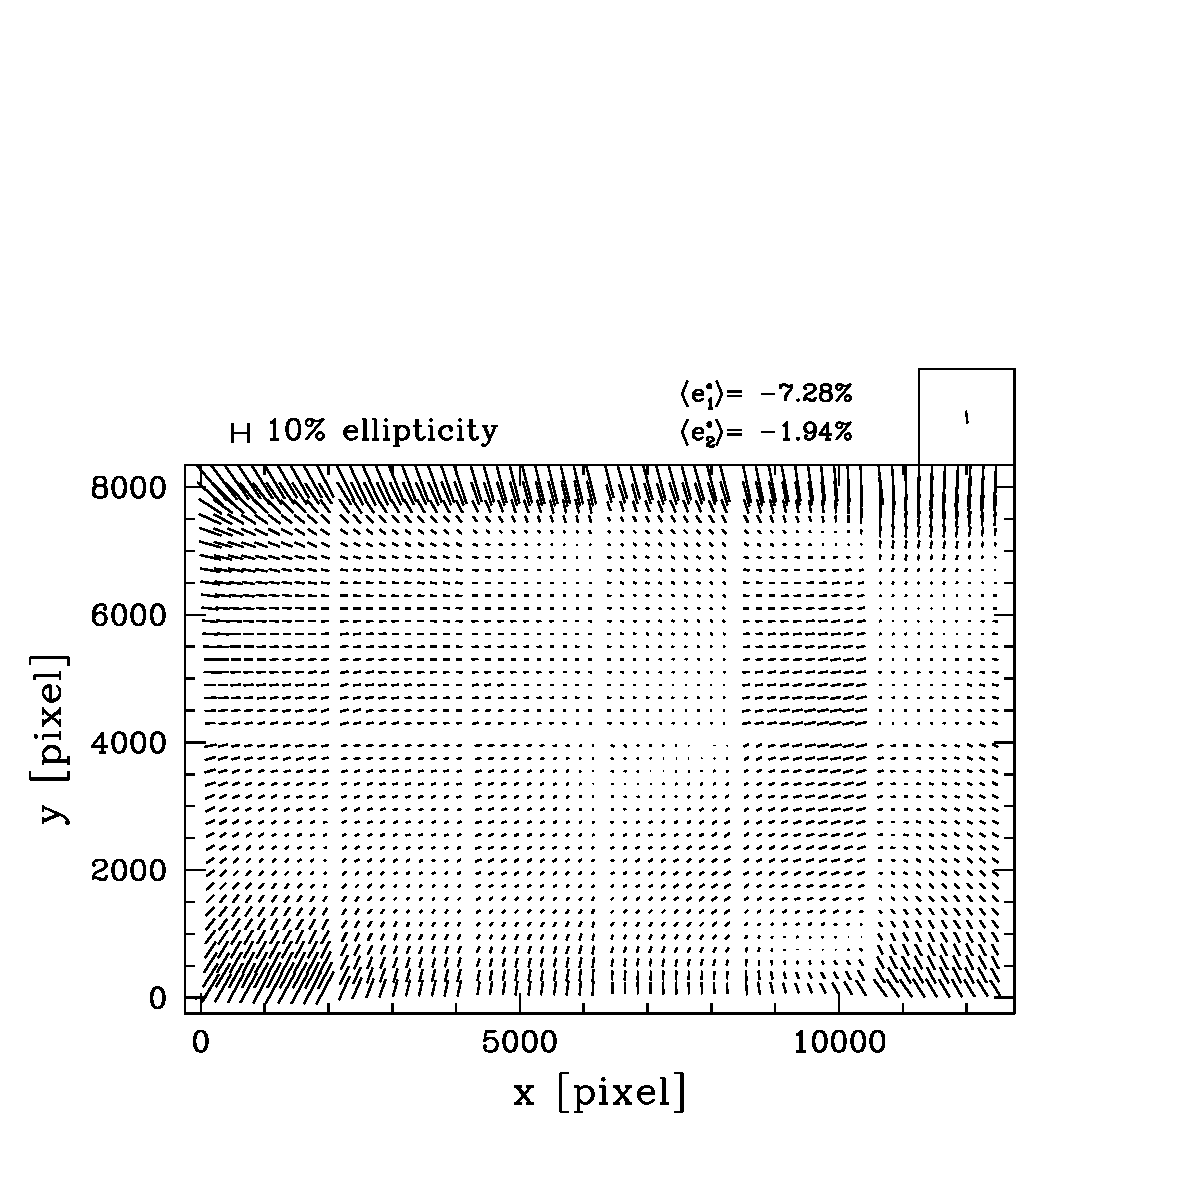
\includegraphics[width=0.5\textwidth]{model.pdf}
	\caption{A visualization of the spatial variation of the PSF ellipticity across the image field, shown as a grid of small vectors indicating the magnitude and orientation of distortions at different pixel positions. Taken from \cite{2004MNRAS.347.1337H}.}
	\label{fig:PSF_space_variability}
\end{figure}

\reviewnote{A section on current PSF models (parametric and data-driven families) is to be added here.}

\section{The observational model}
\label{sec:obsmodel}

Three kinds of variation matter. Spatial variation arises because the path taken by light through the optics depends on the field angle, so the PSF changes with position in the focal plane; this is strongest for wide-field instruments. It is also spatially varying due to the atmosphere being non-uniform in the case of ground based surveys. Spectral variation follows from the wavelength dependence of diffraction (Appendix~\ref{app:optics}) and from chromatic effects in the optics and detector (see section \ref{sec:contributors}). Temporal variation reflects the changing state of the instrument, for example thermal expansion in orbit or, for ground-based telescopes, the evolving atmosphere.

Let $I_{\mathrm{GT}}$ denote the ground-truth intensity of the object of interest (GT for ground truth) and $H_{\mathrm{int}}$ the PSF, written as a function of focal-plane position $(u,v)$, wavelength $\lambda$, time $t$, and the object centroid $(u_i,v_i)$. The observed pixelised image is
\begin{equation}
I_{\mathrm{img}}(\bar u,\bar v;t\mid u_i,v_i)
= F_p\!\left[\int_0^{\infty} T(\lambda)\,(I_{\mathrm{GT}}\star H_{\mathrm{int}})(u,v;\lambda;t\mid u_i,v_i)\,\mathrm{d}\lambda\right]
\circ N(\bar u,\bar v;t\mid u_i,v_i),
\label{eq:obsmodel}
\end{equation}
where $\star$ is convolution, $(\bar u,\bar v)$ are the discrete pixel coordinates, $F_p$ is the degradation operator that samples the continuous image onto the detector grid, and $\circ$ combines the result with the noise term $N$. The function $T(\lambda)$ is the total system transmission. It collects the wavelength-dependent throughput of the mirrors and optics, the transmission of the filter that defines the passband, and the quantum efficiency (QE) of the detector, that is the probability that an incident photon of a given wavelength is converted into a measured photo-electron. The integral over $\lambda$ is needed because $H_{\mathrm{int}}$ depends on wavelength, so a broadband image is a transmission-weighted superposition of monochromatic images, each blurred by its own PSF.

In practice the continuous quantities are inaccessible and the model is discretized. Assuming additive noise and approximating the spectral integral by a sum over $n_\lambda$ bins of width $\Delta\lambda_k$ centred at $\lambda_k$,
\begin{equation}
I_{\mathrm{img}}(\bar u,\bar v;t\mid u_i,v_i)
= F_p\!\left\{\sum_{k=1}^{n_\lambda} T(\lambda_k)\,(I_{\mathrm{GT}}\star H)(\bar u,\bar v;\lambda_k;t\mid u_i,v_i)\,\Delta\lambda_k\right\}
+ N(\bar u,\bar v;t\mid u_i,v_i).
\label{eq:obsmodel_discrete}
\end{equation}

A star is a special case. To good approximation it is a spatial point source with a spectral energy distribution (SED) $f_{(u_i,v_i)}(\lambda)$, so $I_{\mathrm{star}} = \delta(u_i,v_i)\,f_{(u_i,v_i)}(\lambda)$. Substituting this into the model leaves a degraded, noisy sample of the PSF field weighted by the stellar SED. Stars are therefore the data that constrain the PSF model, although their SEDs are usually known only at the low spectral resolution provided by photometric bands.

\section{Contributors to the PSF / PSF model accuracy}
\label{sec:contributors}

The shape of the PSF is set by a long list of physical effects, conventionally split into those that act at the level of the optics, which modify the amplitude and phase of the wavefront, and those that act at the detector, which affect the recorded intensity. A third contribution, the atmosphere, dominates ground-based imaging but is absent for a space telescope such as \textit{Euclid}. We will not consider it in this review.

\subsection{General contributors}
See also ref. \cite{2008A&A...484...67P}.
\begin{itemize}
	\item \textit{The PSF model} the model chosen to describe the PSF will never perfectly describe it.
	\item \textit{The interpolation scheme} no interpolation scheme will exactly describe the PSF as a function of $\vec \theta$. It should be noted that for EUCLID in particular interpolation will no longer be relevant \cite{2020A&A...635A.139E} . EUCLID's PSF is diffraction limited. The PSF thus depends of the spectral energy density (SED) of the galaxy imaged. A physical model of the telescope optics is required to calculate the PSF as a function of SED (and many other parameters). 
	\item \textit{The finite information available from each star} a star provides an image of the PSF that is noisy (photon noise TODO: what is photon noise) and pixelated.
\end{itemize}

\subsection{Optic-level contributors}

For a diffraction limited PSF the most basic contribution is due to finite aperture/lens width. For an unobscured circular aperture of diameter $d$ the PSF is the Airy pattern, whose full width at half maximum (FWHM) is
\begin{equation}
\theta_{\mathrm{FWHM}} = 1.025\,\frac{\lambda}{d},
\label{eq:airy}
\end{equation}
with the first dark ring, the Rayleigh resolution limit, at $1.22\,\lambda/d$. The aperture diameter therefore sets the resolution: a larger aperture gives a narrower PSF.

Real optics depart from the ideal in several ways:
\begin{itemize}
\item \textit{Aberrations.} Imperfect surfaces or alignment cause the wavefront to deviate from the ideal converging sphere. These deviations are encoded in the wavefront error (WFE), introduced through the generalised pupil function in Appendix~\ref{app:optics}, and are usually expanded in Zernike polynomials \cite{noll1976}, which are similar to spherical harmonics but for a disk instead of a sphere.
\item \textit{Surface and polishing errors.} Residual roughness of mirrors and lenses left by manufacturing adds high-spatial-frequency structure to the WFE.
\item \textit{Obscurations.} Internal structure of the telescope can obscure some of the incoming light, modifying the PSF. For Euclid in particular: the secondary mirror and its support structure block part of the pupil and produce characteristic diffraction features, including the spikes seen around bright stars. Because the obscuration is the two-dimensional projection of a three-dimensional structure, its appearance, and hence its imprint on the PSF, depends on the field position. \reviewnote{The strut spikes carry a preferred orientation, so the residual PSF anisotropy they leave can in principle project onto B-modes. Consider linking this to the B-mode discussion elsewhere in the thesis.}
\item \textit{Stray and scattered light.} Light that reaches the detector by unintended paths adds a diffuse component, affecting mostly the faint outer wings of the PSF. TODO: get this a bit clearer.
\item \textit{Contamination.} In the vacuum of outer space materials release trapped / absorbed gasses, this is called molecular outgassing. This can lead to the forming of ice films on optical elements if they are sufficiently cold. This was significant for Gaia and has been studied for Euclid.
\item \textit{Chromatic components.} Elements such as dichroic filters, built from stacks of thin coatings, introduce wavelength-dependent phase and amplitude changes beyond the intrinsic chromaticity of diffraction, even with excellent production quality.
\item \textit{Polarisation.} The scalar treatment of Appendix~\ref{app:optics} neglects polarisation. In reality the optics can partially polarise unpolarised light, and astrophysical foregrounds such as Galactic dust polarize light; both modify the effective PSF and can contribute to WL systematics.
\item \textit{Thermal variation.} Temperature gradients flex the structure and shift the focus, an effect sometimes called breathing. It is more pronounced for space telescopes, although those at the L2 Lagrange point, including \textit{Euclid}, are more stable than telescopes in low Earth orbit.
\end{itemize}

\subsection{Detector-level contributors}

The continuous intensity arriving at the focal plane is sampled by discrete pixels, each integrating the light over its area. Two consequences of this pixellation matter for PSF modelling. First, the continuous image is generally not centred on the pixel grid, so different exposures differ by sub-pixel shifts; comparing a model with an observed star then requires matching their centroids, since otherwise a correct model can still leave a large residual. Second, the sampling may not satisfy the Nyquist--Shannon theorem, which states that a band-limited signal must be sampled at least twice per period of its highest frequency to be reconstructed exactly. For a diffraction limited PSF the relevant scale is set by the highest spatial frequency passed by the aperture, of order $\lambda f/d$ for focal length $f$. \textit{Euclid} is undersampled, so its individual exposures cannot resolve the full PSF. A super-resolution step is required, and a dithering strategy of small sub-pixel pointing offsets between exposures is used to recover well-sampled information.

Further detector effects include:
\begin{itemize}
\item \textit{Optical throughput and CCD QE.} The combined transmission of the optics and filter and the quantum efficiency of the light detectors, i.e. charge-coupled device (CCD), set the total response $T(\lambda)$ in Eq.~\eqref{eq:obsmodel}.
\item \textit{CCD misalignments.} CCDs that do not lie exactly in the focal plane introduce small, chip-dependent defocus.
\item \textit{Guiding errors.} Residual pointing motion (jitter) of the telescope blurs the image and can be modelled as an additional convolution.
\item \textit{Charge transfer inefficiency (CTI).} Radiation damage accumulated in space creates ``traps'' in the electronics of the telescope that delay electrons during readout. Leads to trailing bright sources along the transfer direction.
\item \textit{Brighter-fatter effect (BFE).} Charge already collected in a pixel builds a transverse electric field that deflects later-arriving charge, so bright sources appear broader than faint ones and the response is not linear in flux.
\item \textit{Wavelength-dependent sub-pixel response.} Charge diffuses between neighbouring pixels by an amount that depends on wavelength, adding a chromatic blur.
\end{itemize}

The way exposures are combined also shapes the effective PSF. Coaddition of many exposures raises the signal-to-noise ratio but complicates the PSF, since the combined image has a well-defined PSF only under particular coaddition schemes. Dithering, mentioned above, mitigates undersampling and is especially effective given the stable pointing of a space-based telescope.

\section{Validation of PSF models}
\label{sec:validation}

Validating a PSF model is difficult because the true PSF field is never directly accessible; only noisy star images are available. The basic safeguard is to split the observed stars into an estimation (training) set and a disjoint test (validation) set, for example in an 80/20 ratio, and to assess the model only on the test set. This measures the model's ability to generalise to positions it was not fit to.

\subsection{Pixel-based metrics}

The most direct check is the residual between a predicted and an observed test star. For noiseless simulated stars the root mean square error (RMSE) of the residual measures the reconstruction error directly. For real data the residual is contaminated by noise, so \cite{liaudat2021mccd} introduced metrics that mask the image to its central region, where most of the flux lies, and estimate the noise from the outer region. The leading metric subtracts the noise variance from the masked residual variance, so that a perfect model leaves only noise. Further metrics quantify the mean and the scatter of the residual modeling error. These metrics are useful but, for obvious reasons, hard to translate into actual scientific impact.

\subsection{Moment-based metrics}

Since WL measures galaxy shapes in terms of second order moments, it is natural to characterize the PSF through the same shape statistics. Using definitions of the second moments with some weight function as described in TODO: what to put here. 
A standard estimator is the adaptive-moments algorithm of the HSM (Hirata--Seljak--Mandelbaum) method \cite{hirata_seljak2003}. Several diagnostics are built on these quantities. The shape RMSE is the residual of $e$ and $R^2$ between model and observation; it is simple but says little about the structure of the error.

The meanshapes diagnostic maps the spatial distribution of the ellipticity and size residuals across the focal plane, averaged over many exposures, and reveals spatial patterns that the model fails to capture.

An alternative set of diagnostics are the $\rho$-statistics \cite{rowe2010,jarvis2016}, the auto- and cross-correlations of the PSF ellipticity residual $\delta e_{\mathrm{PSF}}$ and the fractional size residual $\delta R^2_{\mathrm{PSF}}/R^2_{\mathrm{PSF}}$ as functions of angular separation $\theta$,
\begin{align}
\rho_1(\theta) &= \big\langle \delta e_{\mathrm{PSF}}^{*}(\theta')\,\delta e_{\mathrm{PSF}}(\theta'+\theta)\big\rangle, \label{eq:rho1}\\
\rho_2(\theta) &= \big\langle e_{\mathrm{PSF}}^{*}(\theta')\,\delta e_{\mathrm{PSF}}(\theta'+\theta)\big\rangle, \\
\rho_3(\theta) &= \left\langle \left(e_{\mathrm{PSF}}^{*}\tfrac{\delta R^2_{\mathrm{PSF}}}{R^2_{\mathrm{PSF}}}\right)\!(\theta')\,\left(e_{\mathrm{PSF}}\tfrac{\delta R^2_{\mathrm{PSF}}}{R^2_{\mathrm{PSF}}}\right)\!(\theta'+\theta)\right\rangle, \\
\rho_4(\theta) &= \left\langle \delta e_{\mathrm{PSF}}^{*}(\theta')\,\left(e_{\mathrm{PSF}}\tfrac{\delta R^2_{\mathrm{PSF}}}{R^2_{\mathrm{PSF}}}\right)\!(\theta'+\theta)\right\rangle, \\
\rho_5(\theta) &= \left\langle e_{\mathrm{PSF}}^{*}(\theta')\,\left(e_{\mathrm{PSF}}\tfrac{\delta R^2_{\mathrm{PSF}}}{R^2_{\mathrm{PSF}}}\right)\!(\theta'+\theta)\right\rangle, \label{eq:rho5}
\end{align}
where $*$ denotes complex conjugation and $\langle\cdot\rangle$ averages over galaxy pairs at separation $\theta$. Assuming the ellipticity field is statistically isotropic and homogeneous, these depend only on the modulus $|\theta|$. The $\rho$-statistics identify the angular scales on which PSF modelling errors are largest and can be propagated into the shear two-point correlation function (2PCF) to estimate the induced systematic \cite{jarvis2020}.

\section{Change in ellipticity due to PSF}
A derivation of how to actually calculate the change in ellipticity, $\delta e$, due to arbitrary (but reasonably weak) PSF was first given in ref. \cite{1995ApJ...449..460K}. Some errors were then corrected in ref. \cite{1998ApJ...504..636H}. We start with a weighted quadrupole,
\begin{equation}
	Q_{ij}\equiv\int \d^2\theta\;W(\theta)\theta_i\theta_j f(\vec \theta).
\end{equation}
Here $f(\vec \theta)$ is the flux of the image, $W(\theta)$ is a window function, and we work in coordinates such that the dipole vanishes (center of mass coordinates). The PSF is separated into a spherically symmetric part and small but purely anisotropic part. Consider the polarization of an image, $e_\alpha$ given by
\begin{equation}
	e_1\equiv\frac{Q_{11}-Q_{22}}{T}, \quad e_2\equiv\frac{2Q_{12}}{T}, \quad T\equiv Q_{11}+Q_{22}. \label{eq:e_alpha_def}
\end{equation}
These are invariant to the spherically symmetric part (TODO: check if this is actually true) and so we focus only on the anisotropic part. $f$ is changed due to the PSF as
\begin{equation}
	f^{\PSF}(\vec\theta)=(PSF \ast f)(\vec\theta)=\int\d^2\theta'\PSF(\vec\theta')f(\vec \theta-\vec\theta').
\end{equation}
Plugging this into the quadrupole and Taylor expanding gives
\begin{equation}
	\delta Q_{ij}=q_{lm}Z_{lmij},
\end{equation}
where 
\begin{align}
	q_{lm}&\equiv\int d^2\theta\theta_l\theta_m\PSF(\vec\theta),\\
	Z_{lmij}&\equiv\int\d^2\theta W(\theta)\theta_i\theta_j\partial_l\partial_j f(\vec \theta)=\int \d^2\theta f(\vec \theta)z_{lmij},\\
	z_{lmij}&\equiv\frac{\partial\sbr{W(\theta)\theta_i\theta_j}}{\partial_l\partial_m},
\end{align}
where the last line is due to integration by parts. The next step would be to calculate $\delta e_\alpha$, which can ultimately be written as a function of $\delta Q_{ij}$. In the literature a different basis is used, however. Consider that due to the PSF being purely anisotropic $q_{ij}$ must be traceless. Define $p_\alpha$ such that
\begin{equation}
	\begin{bmatrix}
		q_{11} & q_{12} \\ q_{21} & q_{22}
	\end{bmatrix}
	=
	\frac{1}{2}
	\begin{bmatrix}
		p_1 & p_2 \\ p_2 & -p_1
	\end{bmatrix}.
\end{equation}
Then one can relate $\delta e_\alpha$ to $p_\alpha$ through
\begin{align}
\delta e_\alpha&=P^{\PSF}_{\alpha \beta} p_\beta, \\
P^{\PSF}_{\alpha \beta}&\equiv X^{\PSF}_{\alpha \beta} - e_\alpha e^{\PSF}_\beta, \\
X^{\PSF}_{\alpha \beta}&\equiv\frac{1}{T}\int d^2\theta
\left[\begin{array}{cc}
W+2W' \theta^2 + W''(\theta_1^2-\theta_2^2)^2 & 2W''(\theta_1^2-\theta_2^2)
\theta_1\theta_2, \\
2W''(\theta_1^2-\theta_2^2)\theta_1\theta_2 & W+2W' \theta^2 + 4W''\theta_1^2
\theta_2^2,  \\
\end{array}\right]f(\vec\theta), \\
e^{\PSF}_\alpha&\equiv\frac{1}{I_{11}+I_{22}}\int d^2\theta ,
\end{align}
where prime denotes differentiation with respect to $\theta^2$. Again, all that was done here is relating $\delta e_\alpha$ to $\delta Q_{ij}$ and writing out terms explicitly, simply expressed in a different basis.

If the anisotropic part of the PSF is too large compared to the accuracy desired for a survey, one instead has to work non-perturbatively. See reference \cite{2000ApJ...537..555K}.

%--------------------------------------------------------------
\section{Error propagation and requirements}
\label{sec:errorprop}
%--------------------------------------------------------------

To turn these diagnostics into requirements on a model, the PSF errors must be propagated to a bias of the quantity of interest, the galaxy ellipticity / shear. Still working to first order and now assuming an \textit{unweighted} quadrupole definition ($W(\theta)=1$), the error can be written as multiplicative and additive shear bias. The propagation from PSF error to shear bias can be derived in a few steps. First, work with the estimator
	\begin{equation}
		\hat \gamma=\br{P^\gamma}^{-1} e_\alpha, \quad P^\gamma\equiv 2-\langle |\varepsilon_\gal|^2\rangle. \label{eq:shearestimator}
	\end{equation}
	This estimator works because if one expands the flux function inside the quadrupole definition one can find that, at linear order,
	\begin{equation}
		\delta Q_{ij} = G_{ik}Q_{kj}+Q_{ik}G_{kj}, \quad G\equiv\begin{bmatrix}
			\gamma_1 &\gamma_2 \\ \gamma_2 & -\gamma_1
		\end{bmatrix}.
	\end{equation}
	Thus $\delta e_\alpha$ can also be found. Expanding equations \ref{eq:e_alpha_def} gives
	\begin{align}
		\delta \varepsilon_\alpha = 2\gamma_\alpha - 2\varepsilon_\alpha\varepsilon_\beta\gamma_\beta.
	\end{align}
	Averaging both sides and noting that $2\langle \varepsilon_\alpha\varepsilon_\beta \rangle = \delta_{\alpha\beta}\langle |\varepsilon|^2\rangle$ gives equation \ref{eq:shearestimator}.
	
	Second, notice that, in the absence of a window function, the quadrupole of a convolution is the sum of the quadrupoles\footnote{
	Assume that $f$ and $g$ are normalized and have vanishing dipole:
	\begin{align*}
	\int d^2\theta \, f = \int d^2\theta \, g = 1,
	\qquad
	\int d^2\theta \, \theta_i f = \int d^2\theta \, \theta_i g = 0.
	\end{align*}
	Then
	\begin{align*}
	Q_{em}[f * g]
	&= \int d^2\theta \, \theta_e \theta_m \, (f * g)(\boldsymbol{\theta}) \\
	&= \int d^2\theta \, \theta_e \theta_m \int d^2\theta' \, g(\boldsymbol{\theta}') \, f(\boldsymbol{\theta} - \boldsymbol{\theta}') \\
	&= \int d^2\theta \, d^2\theta' \, 
	(\theta_e - \theta'_e + \theta'_e)(\theta_m - \theta'_m + \theta'_m)
	\, g(\boldsymbol{\theta}') \, f(\boldsymbol{\theta} - \boldsymbol{\theta}') \\
	&= \int d^2\theta \, d^2\theta' \,
	(\theta_e - \theta'_e)(\theta_m - \theta'_m)
	\, g(\boldsymbol{\theta}') \, f(\boldsymbol{\theta} - \boldsymbol{\theta}')
	+ \text{(other terms)} \\
	&= Q_{em}[f] + Q_{em}[g] \, .
	\end{align*}
	}, i.e.
	\begin{equation}
		Q_{ij}[f\ast g]=Q_{ij}[f]+Q_{ij}[g], \quad (\text{if }W(\theta)=1).
	\end{equation}
	Combining with equations \ref{eq:e_alpha_def} gives the (lensed) galaxy ellipticity in terms of the PSF ellipticity and observed ellipticity as
	\begin{equation}
		\varepsilon_\gal = \frac{\varepsilon_\obs T_\obs-\varepsilon_\PSF T_\PSF}{T_\obs-T_\PSF}.
	\end{equation}
	Now consider that we have some error in our estimates of $\varepsilon_\PSF$ and $T_\PSF$, denote them as $\delta\varepsilon_\PSF$ and $\delta T_\PSF$. We can then expand $\varepsilon_\gal$ in terms of these quantities to obtain
	\begin{equation}
		\delta\varepsilon_\gal = (\varepsilon_\gal - \varepsilon_\PSF)\frac{\delta T_\PSF}{T_\gal} - \frac{T_\PSF}{T_\gal}\delta\varepsilon_\PSF.
	\end{equation}
	Combining this with the estimator, eq. \ref{eq:shearestimator}, and averaging over a sample of galaxies located in a small enough patch of the sky such that the PSF doesn't change significantly inside of it, gives multiplicative and additive biases
	\begin{align}
		m_\PSF(\vec\theta) &= \frac{\delta T_\PSF(\vec\theta)}{T_\PSF(\vec\theta)},\\
		c_\PSF(\vec\theta) &= -\langle T_\gal^{-1} \rangle \br{P^{\gamma}}^{-1}\sbr{\varepsilon_\PSF\delta T_\PSF+T_\PSF\delta\varepsilon_\PSF}.
	\end{align}
	These biases can then be propagated to $E$ and $B$ mode biases and ultimately into biases of measured cosmological parameters, see section TODO. This is the basis of the PSF model requirements adopted for \textit{Euclid} \cite{laureijs2011,racca2016}, which demand a root mean square error of order $2\times10^{-4}$ on each PSF ellipticity component and of order $10^{-3}$ on the relative PSF size.

The framework has known limitations. It assumes unweighted moments, whereas real measurements use a weight function, which mixes in higher-order moments so that even in the absence of noise the second-order moments are affected. More significantly, a diffraction-limited PSF, such as \textit{Euclid}'s, has a complex shape that its second-order moments do not describe well. The error in the higher moments of the PSF (the higher moments error, HME) then contributes to the shear bias and is missed by the standard framework. \cite{zhang2021} showed that it can be a significant source of systematics for upcoming surveys. The requirements above should therefore be applied with care for diffraction-limited instruments.

A promising direction is to make the entire forward model differentiable. Automatic differentiation \cite{baydin2017} computes exact derivatives of a model output with respect to its parameters by applying the chain rule through the computation, without deriving gradients by hand. A forward model that is differentiable from the wavefront parameters through to the target estimator would supply the derivatives needed for error propagation directly, and would allow more complex scenarios to be treated than the analytic moment-based expansion permits. This idea underlies recent differentiable optical PSF models \cite{liaudat2023wavediff}.

TODO: relation to $B$-modes? Check if there is some work on this.

TODO: make biases and resulting spectra a general section, because now both masking and PSF errors are expressed as biases

\section{Modern PSF models}
Relevant for Euclid:
\begin{itemize}
	\item Euclid VIS parametric model. Parametric. Official model.
	\item WaveDiff. Data-driven. Made for Euclid. Handles chromaticity and super resolution. Basically tries to estimate $W$ function from earlier.
	\item Resolved component analysis. Modern version of interpolation / optimization problem.
\end{itemize}

\chapter{Modelling Galaxy B-modes}
\section{Masking / window function effects}
\subsection{Modification to shear}
Given a set of observed galaxies, the shear field is given by
\begin{equation}
	\gamma(\hat n)=\sum_{g\in\text{ observed gals}} e_g \delta(\hat n - \hat n_g),
\end{equation}
here $e_g$ is the ellipticity of the galaxy. Now assume the most general version of masking, which is a window function $W(\hat n)$, i.e. at $\hat n$ only a fraction $W(\hat n)$ of the surveyed galaxies are taken into account\footnote{Or, alternatively, they are weighed by a factor $W(\hat n)$.} The observed shear is then
\begin{equation}
	\gamma^{\text{obs}}(\hat n) = W(\hat n)\gamma(\hat n).
\end{equation}
In spherical harmonic space this gives
\begin{align}
	\gamma_{\ell m}^{\text{obs}} &= \int \d^2\Omega \; _2Y_{\ell m}^*(\hat n)W(\hat n)\gamma(\hat n)\\
	&= \int \d^2\Omega \; _2Y_{\ell m}^*(\hat n)W(\hat n)\br{\sum_{\ell' m'} \;_2Y_{\ell'm'}(\hat n)\gamma_{\ell'm'}}\\
	&= \sum_{\ell' m'} \br{\int \d^2\Omega \; _2Y_{\ell m}^*(\hat n)W(\hat n)_2Y_{\ell'm'}(\hat n)} \gamma_{\ell'm'}. \label{eq:windowedshearfunc}
\end{align}

I.e. just a matrix multiplication of the true multipole moments. $_nY_{\ell m}$ is the spin $n$ spherical harmonic.
\subsection{Effects from uncertainty in the window function}
In theory one could simply solve the system of equations shown in equation \ref{eq:windowedshearfunc}. In practice the window function is not perfectly known, %TODO: maybe explain why? I don't really get why it can't be perfectly known
 leading to bias in estimated shear. This is discussed in reference \cite{2019OJAp....2E...5K}, among others. The reasoning proceeds as follows. Assume multiplicative and additive bias to the shear, i.e.
 \begin{equation}
 	\gamma^{\text{obs}}(\hat n)=\sbr{1+m(\hat n)}\gamma(\hat n) + c(\hat n).
 \end{equation}
 A spherical harmonic transform as done to obtain equation \ref{eq:windowedshearfunc} gives
 \begin{align}
 	\gamma^{E,\text{obs}}_{\ell m} &= \gamma^E_{\ell m} + \sum_{\ell'm'}\sbr{\gamma^E_{\ell'm'}W^+_{\ell\ell' m m'} + \gamma^B_{\ell' m'}W^-_{\ell\ell' m m'}} + c^E_{\ell m}, \\
 	\gamma^{B,\text{obs}}_{\ell m} &= \gamma^B_{\ell m} + \sum_{\ell'm'}\sbr{\gamma^B_{\ell'm'}W^+_{\ell\ell' m m'} - \gamma^E_{\ell' m'}W^-_{\ell\ell' m m'}} + c^B_{\ell m}. 
 \end{align}
 Here
 \begin{align}
 	W^+_{\ell\ell'mm'} &\equiv \frac{1}{2}\sbr{_2W_{\ell\ell'mm'} + \;_{-2}W^*_{\ell\ell'mm'}}, \\
  	W^+_{\ell\ell'mm'} &\equiv \frac{i}{2}\sbr{_2W_{\ell\ell'mm'} - \;_{-2}W^*_{\ell\ell'mm'}},
 \end{align}
 and
 \begin{equation}
 	_sW_{\ell\ell'mm'}\equiv\int \d^2\Omega \;_sY^*_{\ell'm'}(\hat n)m(\hat n)\,_sY_{\ell m}(\hat n).
 \end{equation}
 It is immediately clear that there is mixing between $E$ and $B$ modes, in particular, $B$ modes will be observed even if they are not present in the true shear field.
 The next question is how the power spectra are changed. We work with the usual definition
 \begin{equation}
 	C^{XY, \text{obs}}_{\ell} = \frac{1}{2\ell+1}\sum_m \gamma^{X,\text{obs}}_{\ell m} \gamma^{Y,\text{obs}}_{\ell m}, \quad X,Y\in\{E,B\},
 \end{equation}
and assume $C^{EB}_\ell = 0$. This gives a lengthy set of equations, see equation 7 of \cite{2019OJAp....2E...5K}\footnote{They also include a constant multiplicative bias term, $m_0$. I.e. $\gamma^{\text{obs}}(\hat n)=\sbr{1+m_0+m(\hat n)}\gamma(\hat n) + c(\hat n)$. Clearly our explanation is still completely general, as $m_0$ could always be absorbed into $m(\hat n)$.}. If we assume the bias terms are small and work to linear order in them, then the equations simplify considerably.
\begin{align}
	C^{EE,\text{obs}}_\ell &=(1+2\langle \text{Re}\sbr{m(\hat n)}\rangle)C^{EE}_\ell + 2C^{c_EE}_\ell, \\ 
	C^{EB,\text{obs}}_\ell &=-\langle \text{Im}\sbr{m(\hat n)}\rangle)C^{EE}_\ell + \langle \text{Re}\sbr{m(\hat n)}\rangle)C^{BB}_\ell+ 2C^{c_EB}_\ell, \\
	C^{BB,\text{obs}}_\ell &=(1+2\langle \text{Re}\sbr{m(\hat n)}\rangle)C^{EE}_\ell + 2C^{c_BB}_\ell.
\end{align}
Here $C^{c_XY}_\ell$ is just the power spectrum with $c^X_{\ell m}$ moments instead of $\gamma^X_{\ell m}$.

\section{$B$-modes due to intrinsic alignment}


\section{Lensing corrections (post-Born)}
\subsection{Leading-order formulas}
\label{sec:leading_order}

Following \cite{Krause_2010}, we work in the flat-sky approximation with the sky in the $xy$-plane and photons propagating along $-\hat{\mathbf{z}}$. We set $c=1$ so that the Newtonian potential $\Phi$ is dimensionless. Lower-case Roman indices $a,b,\ldots \in \{1,2\}$ label Cartesian components; capital Roman indices $I,J,\ldots \in \{1,2\}$ label polar (shear/ellipticity) components; Greek indices label tomographic redshift slices.

To first order in $\Phi$, the photon geodesic is integrated along the unperturbed ray (the Born approximation). The Jacobian of the resulting mapping defines the distortion tensor $\psi_{ij} \equiv \delta_{ij} - \partial n_i/\partial n_{0j}$, which encodes convergence, shear, and rotation via $\kappa = \tfrac{1}{2}(\psi_{11}+\psi_{22})$, $\gamma_1 = \tfrac{1}{2}(\psi_{11}-\psi_{22})$, $\gamma_2 = \tfrac{1}{2}(\psi_{12}+\psi_{21})$, and $\omega = \tfrac{1}{2}(\psi_{12}-\psi_{21})$.

Introducing the angular Fourier transform of the potential \cite{2005PhRvD..72h3001D},
\begin{equation}
    \tilde{\phi}(\mathbf{l};\chi) \equiv \frac{1}{\chi^2}\int\frac{\d k_3}{2\pi}\,\tilde{\Phi}(\mathbf{l}/\chi,k_3;z(\chi))\,e^{ik_3\chi},
\end{equation}
the first-order convergence and shear read
\begin{equation}
    \tilde{\kappa}^{(1)}(\mathbf{l},z_s) = -l^2\int_0^{\chi_s}\!\d\chi\, W(\chi,\chi_s)\,\tilde{\phi}(\mathbf{l};\chi),\qquad \tilde{\gamma}_I^{(1)}(\mathbf{l},z_s) = T_I(\mathbf{l})\,\tilde{\kappa}^{(1)}(\mathbf{l},z_s),
\end{equation}
with lensing kernel $W(\chi',\chi) = (1/\chi' - 1/\chi)\,\Theta(\chi-\chi')$, source distance $\chi_s = \chi(z_s)$, and $T_1(\mathbf{l}) = \cos(2\varphi_\mathbf{l})$, $T_2(\mathbf{l}) = \sin(2\varphi_\mathbf{l})$. The E/B decomposition
\begin{equation}
    \tilde{\gamma}_E(\mathbf{l},z_s) = \delta_{IJ}T_I(\mathbf{l})\,\tilde{\gamma}_J(\mathbf{l},z_s),\qquad \tilde{\gamma}_B(\mathbf{l},z_s) = \epsilon_{IJ}T_I(\mathbf{l})\,\tilde{\gamma}_J(\mathbf{l},z_s)
\end{equation}
yields the leading-order identities $\tilde{\gamma}_E^{(1)} = \tilde{\kappa}^{(1)}$ and $\tilde{\gamma}_B^{(1)} = \tilde{\omega}^{(1)} = 0$: linear lensing is curl-free and produces no B-mode power.

Under the Limber approximation \cite{1992ApJ...388..272K}, the leading tomographic cross-spectra for $z_\alpha \le z_\beta$ take the standard form
\begin{equation}
    C^{(11)}_{\tilde{\gamma}_E}(l;z_\alpha,z_\beta) = C^{(11)}_{\tilde{\kappa}}(l;z_\alpha,z_\beta) = l^4\int_0^{\chi_\alpha}\!\d\chi\,\frac{W(\chi,\chi_\alpha)W(\chi,\chi_\beta)}{\chi^2}\,P_\Phi(l/\chi;z(\chi)),
\end{equation}
with $C^{(11)}_{\tilde{\gamma}_B} = C^{(11)}_{\tilde{\omega}} = 0$. The superscript $(11)$ denotes two first-order fields, i.e.\ the $\mathcal{O}(\Phi^2)$ contribution.

The observable is the mean galaxy ellipticity, which estimates the reduced shear $g_I \equiv \gamma_I/(1-\kappa)$,
\begin{equation}
    \langle e_I\rangle = C\,\frac{\gamma_I}{1-\kappa},
    \label{eq:ellipticity_reduced_shear}
\end{equation}
where $C$ depends on the ellipticity estimator and source population \cite{1995A&A...294..411S,1997A&A...318..687S}. In the limit $\kappa, |\gamma| \ll 1$ this reduces to $\gamma_I$, and ellipticity two-point statistics reduce to the shear power spectrum above. The corrections discussed in the remainder of this chapter enter at $\mathcal{O}(\Phi^3)$ or higher and spoil these clean identities --- in particular, they source a non-vanishing galaxy B-mode.

\subsection{Higher order corrections}
Going back to the perturbed FLRW metric, a photon will of course follow its null geodesic equation,
\begin{equation}
	\frac{\d }{\d\chi}\br{\frac{\d\vec n}{\chi}\chi}=-2\frac{\partial \Phi(\vec x(\vec n, \chi);z(\chi))}{\partial\vec n}\chi. \label{eq:photon_geodesic}
\end{equation}
The leading order equations take $\vec x(\vec n, \chi) \approx\vec x^{(1)}(\vec n, \chi)=\vec n_0 \chi$. We can define the deflection angle $\vec d \equiv \vec n - \vec n_0$ and enforce the appropriate initial conditions ($\vec n(\chi=0)=\vec n_0$ and $\partial_\chi \vec n(\chi = 0)=0$). Then Taylor expand the potential in equation \ref{eq:photon_geodesic} in terms of the deflection angle and around the unperturbed path, i.e.
\begin{equation}
	\Phi(\vec x(\vec n, \chi);z(\chi)) = \Phi(\vec n_0\chi;z(\chi))+\Phi_{,a}(\vec n_0\chi;z(\chi)) d_a(\chi) + \frac{1}{2}\Phi_{,ab}(\vec n_0\chi;z(\chi))d_a(\chi)d_b(\chi) +\cdots.
\end{equation}
Higher order corrections are then obtained by iteratively solving order by order in $\vec d(\chi)$. For ``next to leading order'' corrections to the power spectra one needs to work to 3rd order in $\vec d$. The corrections consist of ``$(22)$'' and ``$(13)$'' power spectra. Naively, one would expect the next to leading order term to be of the type $(12)$, however under the Limber approximation this vanishes. What then follows is working out all terms, Fourier transforming, separating into $E$ and $B$ modes, creating the power spectra, and applying the Limber approximation. The steps are straightforward but require a lot of algebra. They are displayed in \cite{Krause_2010}, the final result is presented in their tables 1 and 2. 
\begin{table*}[t]
\tiny
\centering
\caption{$\mathcal{O}(\Phi^4)$ contributions to the reduced shear B-mode power spectrum, reproduced from \cite{Krause_2010}. All power spectra carry redshift indices $z_\alpha, z_\beta$. The auxiliary quantities $M$, $W$, $T_\kappa$, and the angles $\varphi_{\mathbf{l}}$ are defined in the text.}
\label{tab:B_mode_corrections}
\renewcommand{\arraystretch}{1.8}
\begin{tabular}{p{0.3\textwidth} p{0.7\textwidth}}
\hline\hline
Term & Contribution to $C_{\tilde{g}_B}(l)$ \\
\hline
$\left\langle \tilde{\gamma}_B^{(2)}(\vec{l}, z_\alpha)\, \tilde{\gamma}_B^{(2)}(\vec{l}'', z_\beta) \right\rangle$
& $\displaystyle 4 l^2 \int \frac{\d^2 \vec{l}'}{(2\pi)^2} \left( l' \sin \varphi_{\vec{l}'} \right)^2 \left[ \vec{l}' \cdot (\vec{l} - \vec{l}') \right]^2 M\!\left( l', |\vec{l} - \vec{l}'|; z_\alpha, z_\beta \right)$ \\

$\left\langle \tilde{\gamma}_B^{(2)}(\vec{l}, z_\alpha) \left( \tilde{\gamma}^{(1)} * \tilde{\kappa}^{(1)} \right)_B (\vec{l}'', z_\beta) \right\rangle$
& $\displaystyle -2 \int \frac{\d^2 \vec{l}'}{(2\pi)^2} \left[ \vec{l}' \cdot (\vec{l} - \vec{l}') \right] |\vec{l} - \vec{l}'|^2 \, l\, l'^3 \sin \varphi_{\vec{l}'} \left\{ \sin(2\varphi_{\vec{l}'}) + \sin(2\varphi_{\vec{l} - \vec{l}'}) \right\}$
\newline
$\displaystyle \times \int_0^{\chi_\beta} \!\d\chi\, \frac{W(\chi, \chi_\alpha)\, W(\chi, \chi_\beta)}{\chi^2} \int_0^{\chi} \!\d\chi'\, \frac{W(\chi', \chi_\beta)\, W(\chi', \chi)}{\chi'^2} P_\Phi(l'/\chi; z(\chi))\, P_\Phi(|\vec{l} - \vec{l}'|/\chi'; z(\chi'))$ \\

$\left\langle \left( \tilde{\gamma}^{(1)} * \tilde{\kappa}^{(1)} \right)_B (\vec{l}, z_\alpha) \left( \tilde{\gamma}^{(1)} * \tilde{\kappa}^{(1)} \right)_B (\vec{l}'', z_\beta) \right\rangle$
& $\displaystyle \int \frac{\d^2 \vec{l}'}{(2\pi)^2} \sin(2\varphi_{\vec{l}'}) \Big\{ \left[ \sin(2\varphi_{\vec{l}'}) + \sin(2\varphi_{\vec{l}' - \vec{l}}) \right] C^{(11)}_{\tilde{\gamma}_E}(l'; z_\alpha, z_\beta)\, C^{(11)}_{\tilde{\gamma}_E}(|\vec{l}' - \vec{l}|; z_\alpha, z_\beta)$
\newline

$\displaystyle + \int \frac{\d^2 \vec{l}'''}{(2\pi)^2} \sin(2\varphi_{\vec{l}'''})\, T_\kappa(\vec{l}', \vec{l} - \vec{l}', \vec{l}''', -\vec{l} - \vec{l}'''; z_\alpha, z_\alpha, z_\beta, z_\beta) \Big\}$ \\
\hline
\end{tabular}
\end{table*}
The quantities appearing in Table~\ref{tab:B_mode_corrections} are defined as follows. The lensing kernel is
\begin{equation}
    W(\chi', \chi) = \left( \frac{1}{\chi'} - \frac{1}{\chi} \right) \Theta(\chi - \chi'),
\end{equation}
with $\Theta$ the Heaviside step function and $\chi_\alpha \equiv \chi(z_\alpha)$ the comoving distance to source slice $\alpha$. Azimuthal angles of 2D Fourier modes are denoted $\varphi_{\mathbf{l}}$, so that $\mathbf{l} = l(\cos\varphi_{\mathbf{l}}, \sin\varphi_{\mathbf{l}})$; all results are written in the convention $\mathbf{l} \parallel \hat{\mathbf{x}}$, which is permissible since the power spectra depend only on $l = |\mathbf{l}|$.

The mode-coupling integral $M$ encodes the lens-lens coupling characteristic of multiple-deflection corrections,
\begin{equation}
    M(l, l'; z_\alpha, z_\beta) = \int_0^{\chi_\alpha} \!\d\chi\, \frac{W(\chi, \chi_\alpha)\, W(\chi, \chi_\beta)}{\chi^2} \int_0^{\chi} \!\d\chi'\, \frac{W^2(\chi', \chi)}{\chi'^2}\, P_\Phi(l/\chi; z(\chi))\, P_\Phi(l'/\chi'; z(\chi')).
\end{equation}

The tomographic convergence trispectrum $T_\kappa$ is the Limber projection of the 3D matter-density trispectrum,
\begin{align*}
    T_\kappa(\mathbf{l}_1, \mathbf{l}_2, \mathbf{l}_3, -\mathbf{l}_{123}; z_\alpha, z_\beta, z_\gamma, z_\delta) &= \left( \frac{3}{2} \Omega_m H_0^2 \right)^4 \int \!\d\chi\, \frac{W(\chi, \chi_\alpha)\, W(\chi, \chi_\beta)\, W(\chi, \chi_\gamma)\, W(\chi, \chi_\delta)}{\chi^6} \\\ 
    &\times\left(1 + z(\chi)\right)^4 T(\mathbf{l}_1/\chi, \mathbf{l}_2/\chi, \mathbf{l}_3/\chi, -\mathbf{l}_{123}/\chi; z(\chi)),
\end{align*}
where $\mathbf{l}_{123} \equiv \mathbf{l}_1 + \mathbf{l}_2 + \mathbf{l}_3$ and the 3D matter trispectrum $T(\mathbf{k}_1, \mathbf{k}_2, \mathbf{k}_3, \mathbf{k}_4)$ is the connected part of the four-point function,
\begin{equation}
    \left\langle \tilde{\delta}(\mathbf{k}_1)\, \tilde{\delta}(\mathbf{k}_2)\, \tilde{\delta}(\mathbf{k}_3)\, \tilde{\delta}(\mathbf{k}_4) \right\rangle_c = (2\pi)^3\, \delta_D(\mathbf{k}_1 + \mathbf{k}_2 + \mathbf{k}_3 + \mathbf{k}_4)\, T(\mathbf{k}_1, \mathbf{k}_2, \mathbf{k}_3, \mathbf{k}_4).
\end{equation}
\cite{Krause_2010} evaluate $T_\kappa$ using the halo-model prescription of \cite{2001ApJ...554...56C}, which splits the trispectrum into one-, two-, three-, and four-halo contributions. On the angular scales relevant for Stage-IV surveys the Gaussian (disconnected) piece dominates, and in the halo-model framework the connected contribution to the B-mode spectrum is further suppressed by the angular projection factors relative to the E-mode.

\section{$B$-modes due to galaxy clustering}
From \cite{Schneider_2002}. In the presence of a galaxy correlation function $\delta_{\mathrm D}(z_1-z_2)g(z_1;\theta_1)$ ($\theta = |\vec\theta_1-\vec\theta_2|$) we get a modified source redshift distribution of pairs of galaxies at redshifts $z_1$ and $z_2$, i.e.
\begin{equation*}
    p(z_1, z_2;\theta) = \frac{p(w_1;\theta)p(w_2;\theta)[1+\delta_{\mathrm D}(w_1-w_2)g(w_1;\theta)]}{1+\omega(\theta)},
\end{equation*}
where
\begin{equation*}
    \omega(\theta) = \int_0^\infty\mathrm d z \; p(z;\theta)^2g(z;\theta).
\end{equation*}

Defining ratio of distance to source and distance from redshift $z$ to source as
\begin{equation*}
    R(z,z_s)=\frac{\chi(z_s)-\chi(z)}{\chi(z_s)},
\end{equation*}
one can obtain the following equation in configuration space (eq 49 of \cite{Schneider_2002})
\begin{equation*}
    \xi_\pm = \left ( \frac{3H_0^2\Omega_0}{2c^2} \right )^2\int_0^\infty \frac{\mathrm d z}{a^2(z)}\int\frac{\mathrm d \ell \; \ell}{2\pi}P_\delta\left ( \frac{\ell}{\chi(z)},z \right ) J_{0,4}(\ell \theta)\langle R(z, z_1)R(z,z_2) \rangle.
\end{equation*}

The $R(\cdot, \cdot)$ correlation is then modified due to galaxy clustering as
\begin{equation*}
    \langle R(z, z_1)R(z,z_2) \rangle = \frac{W^2(z)+V(z,\theta)}{1+\omega(\theta)},
\end{equation*}
where
\begin{align*}
    W(z) &= \int_z^\infty \mathrm z_1 \; p(z_1)\frac{\chi(z_1)-\chi(z)}{\chi(z_1)} \\
    V(w, \theta) &= \int_z^\infty \mathrm d z_1 \; p^2(z_1) \left ( \frac{\chi(z_1)-\chi(z)}{\chi(z_1)} \right )^2 g(z_1; \theta)
\end{align*}
Clustering thus introduces $V(\cdot,\cdot)$, which leads to $B$-modes (and corrections to $E$-modes).

To get the $B$-modes, first define
\begin{align*}
    P_{\kappa}(\ell) &= \left ( \frac{3H_0^2\Omega_0}{2c^2} \right )^2 \int_0^\infty \frac{\mathrm d z}{a^2(z)} W^2(z)P_\delta \left (\frac{\ell}{\chi(z)}, z \right ) ,\\
    P_{c}(\ell, \theta) &= \left ( \frac{3H_0^2\Omega_0}{2c^2} \right )^2 \int_0^\infty \frac{\mathrm d z}{a^2(z)} V(z, \theta)P_\delta \left (\frac{\ell}{\chi(z)}, z \right ).
\end{align*}
Then define
\begin{equation*}
    \mathcal P(\ell, \theta)= \frac{P_c(\ell,\theta) - w(\theta)P_{\kappa}(\ell)}{1+\omega(\theta)}.
\end{equation*}
One then obtains (eq 60 from \cite{Schneider_2002}) 
\begin{equation*}
    P_B(\ell)=\frac{1}{2}\int\mathrm d \theta\;\theta \int \mathrm d \ell' \; \ell' \mathcal P(\ell'; \theta)[J_0(\ell\theta)J_0(\ell'\theta)\pm J_4(\ell\theta)J_4(\ell'\theta)].
\end{equation*}

\section{$B$-modes due to flux / size cutoffs and lensing}
(TODO: Check \cite{Bartelmann_2001}, also check Schmidt et al. 2008; Hui et al. 2007 as cited in \cite{Krause_2010} for effects on bispectrum/3-point.) Galaxies are selected based on brightness and size cutoffs. This leads to magnification bias and size bias. This gives B-mode correction. See eq. 60 of \cite{Krause_2010}. On scales $\ell>50$ lensing bias effectively increases the B-mode power spectrum by approximately a factor $(1 + 2q)$, where $q$ is determined by the slope of the luminosity and radius distribution functions of the galaxy sample.

If we work with a flux and size cutoff and define \cite{Schmidt_2009}
\begin{equation*}
    q=-2\frac{\partial \ln n_{\text{obs}}}{\partial \ln f}|_{r_{\min}, f_{\min}} - \frac{\partial \ln n_{\text{obs}}}{\partial \ln r}|_{r_{\min}, f_{\min}} - 2,
\end{equation*} then (at 2nd order in lensing)
\begin{equation*}
    1+\delta_{\text{lens}} = \frac{1+q\kappa^2 + C_1\kappa^2+C_2|\gamma|^2}{1+C_1\langle \kappa^2\rangle + C_2\langle |\gamma|^2\rangle}.
\end{equation*}
The measured reduced shear $g_{\text{obs}}$ is given in terms of the actual reduced shear $g$, through $g_{\text{obs}}=g(1+\delta_{\text{lens}})$. This corrected value is then correlated to obtain B-modes.

TODO: okay so this is multiplicative bias then? Express in that language.

\chapter{Calibration and Validation with Simulations}
TODO here:
\begin{enumerate}
    \item Explain validity of EFT of IA based on \cite{bakx2023effectivefieldtheoryintrinsic}
    \item Take a look at hydrodynamic simulations \cite{Samuroff_2021, Johnston_2023}
\end{enumerate}


\printbibliography

\appendix

\chapter{Simulating/modeling nonlinear structure formation and baryonic feedback with HMCODE}
\section{The halo model}
In order to accurately model the matter power spectrum at nonlinear scales, the halo model has been proposed since the early 2000's (TODO: ESSENTIAL REFERENCES HERE). One assumes that all matter is located in exactly one halo. First rewrite the matter density field in the dimensionless quantity $\Delta^2$:
\begin{equation}
    \Delta^2(k) = 4\pi V\br{\frac{k}{2
    \pi}}P(k),
\end{equation}
which gives the fractional contribution to the variance per logarithmic interval in $k$.
In the halo model, the power spectrum can be split into correlations between points within the same halo and between points within different halos. This gives the 1 and 2 halo terms, respectively.
\begin{equation}
    \Delta^2(k)=\Delta^2_{2H}+\Delta^2_{1H}.
\end{equation}
The 1 halo term is given as
\begin{equation}
    \Delta^2_{1H}(k) = 4\pi\br{\frac{k}{2\pi}}^3\frac{1}{\bar\rho^2}\int_{0}^\infty M^2 W^2(k, M)F(M)\d M.
\end{equation}
The following definitions are in order:
\begin{enumerate}
    \item $F(M)$ is the halo mass function, it is defined so that $F(M)\d M$ is the comoving number density of halos with mass between $M$ and $M + \d M$.
    \item $W(k, M)$ is the normalized Fourier transform of the halo density profile, $\rho_{halo}(r, M)$, which is assumed to be spherically symmetric:
    \begin{equation}
        W(k,M) = \mathcal F[\frac{1}{M}\rho_{halo}(r,M)](k) = \frac{1}{M}\int_0^{r_v}\frac{\sin(kr)}{kr}4\pi r^2\rho_{halo}(r, M) \d r.
    \end{equation}
    \item $r_v$ is the virial radius, defined such that the average density within a distance $r_v$ from the center of the halo is $\Delta_v \bar\rho$, where $\Delta_v$ is chosen by the author and is usually around 200.
\end{enumerate}
TODO: 2 halo spectrum def?

To get the halo model to work we then need to choose an accurate halo density profile. A common one is the NFW profile \cite{Navarro_1997},
\begin{equation}
    \rho_{NFW}(r) = \frac{\rho_N}{(r/r_s)(1+r/r_s)^2},
\end{equation}
where $r_s$ is the scale that roughly separates the core of the halo from the outer portion and $\rho_N$ is a normalization constant. The other choice that needs to be made is for the halo number density. It has been shown to have a near univeral form (TODO: SOME REFS). First define
\begin{equation}
    v \equiv \frac{\delta_c}{\sigma(M)},
\end{equation}
where $\sigma(M)$ is the variance of the mass density smoothed on the comoving scale $r_v$ corresponding to a halo of mass $M$ and $\delta_c$ at some redshift $z$ is defined through the linear growth function and deviation function $\sigma$.

Now define $f(v)$ so that it relates to $F(v)$ as 
\begin{equation}
    \frac{M}{\bar \rho}F(M)\d M = f(v) \d v.
\end{equation}
$f$ then has a nearly universal which was first derived in \cite{1974ApJ...187..425P} and improved upon in \cite{Sheth_1999} to better fit simulations. It is given as
\begin{equation}
    f(v) = A_f\sbr{1+\frac{1}{(av^2)^p}}e^{-av^2/2}, \quad a = 0.707, \quad p = 0.3.
\end{equation}
It is accurate up to about 20 percent for a wide range of cosmologies.

\section{Baryonic feedback}
Baryonic feedback refers to effects unique to baryons due to their collisional and warm nature. Important effects include cooling, supernova explosions, and active galactic nuclei (AGN). (TODO: ADD BASIC REFS)
\begin{enumerate}
    \item Baryonic matter has inelastic collisions. Kinetic energy is lost and converted mainly into heat, which is then converted into radiative energy. This causes baryonic matter to clump up more than CDM, in turn leading to the creation of macroscopic structures such as stars and planets, as well as to denser halo cores than expected from a CDM only universe.
    \item Active galactic nuclei means a galaxy with an active ("feeding") supermassive black hole at its center. Matter is sucked into accretion disks, where it is heated up. This releases a large amount of energy in the form of radiation and jets (relativistic plasma) back into the halo, thereby expanding ("bloating") it. AGN feedback can reduce the baryon fraction in the centres of haloes by a factor of 2 in the most extreme models \cite{Duffy_2010}.
    \item Supernova explosions have essentially the same effect on halo structure. Energy is released into the halo in the form of radiation, heating up the halo and bloating it.
\end{enumerate}
Constraints from the Dark Energy Survey could be strongly biased if the most extreme feedback scenarious apply and constraints from Euclid would be severely biased for any feasible feedback scenario. The halo model is particularly good at taking into account baryonic feedback, as its main effect is to change halo shape, which we can easily change when using this model, \cite{Duffy_2010, Semboloni_2011, mohammed2014baryoniceffectsweaklensingtwopoint}.




\section{Optimizing the halo model and taking into account baryonic feedback}
The halo model has been significantly improved upon by adding degrees of freedom and fitting to simulations in \cite{Mead_2016} and later with improved accuracy in \cite{Mead_2021}. In particular, they take into account BAO damping, massive neutrinos and baryonic feedback. The key changes made are:
\begin{enumerate}
    \item For the 2 halo term, they use ``de-wiggled'' linear theory. The BAO ``wiggles'' are isolated from the rest of the power spectrum signal,
    \begin{equation}
        P^{lin}(k,z) = P_{smt}(k,z) + P_{wig}(k,z)
    \end{equation}
    then the de-wiggled linear power spectrum has the BAO wiggles damped at small scales by removing part of that contribution as follows:
    \begin{equation}
        P_{dwl}(k,z) = P^{lin}(k,z) - (1-e^{-k^2\sigma_{v}(z)})P_{wig}(k,z).
    \end{equation}
    This damping models the BAO damping that occurs due to non-linear evolution. 2 halo term is then given in terms of this de-wiggled power spectrum. The full 2 halo equation (TODO: REF THE EQ ONCE I WRITE IT DOWN) would likely be more accurate but is significantly more costly to compute due to it containing an integral.
    \item In order to obtain an accurate approximation of the 2 halo term, further damping of the power spectrum as a whole is required on smaller scales. Nonlinear collapse transfers power from large and intermediate scales into very small scales, causing a slight  suppression at $k\sim 0.03, z=0$ and an enhancement at high $k$. This suppression is modeled as
    \begin{equation}
        P^{2H}(k,z) = P_{dwl}(k,z)\sbr{1-f\frac{(k/k_d)^{n_d}}{1+(k/k_d)^{n_d}}},
    \end{equation}
    where $f$, $n_d$, and $k_d$ are free parameters.
    \item On large scales the 1 halo term is too large and actually outgrows the linear / 2 halo term. This is because halos are assumed to be randomly distributed over space, which leads to a poisson noise contribution. In reality, they are much more uniformly distributed and are not allowed to overlap with one another due to how the halo model is constructed. Damping factor at large scales is thus required to compensate for this deficiency. This is done as
    \begin{equation}
        P^{1H}(k,z)\rightarrow P^{1H}(k,z) \frac{(k/k_*)^4}{1+(k/k_*)^4},
    \end{equation}
    where $k_*$ is another free parameter.
    \item To take into account halo bloating, e.g. from baryonic feedback, the halo mass distribution is modified in a mass dependent way as
    \begin{equation}
        \rho (r, M) \propto \frac{1}{r/(v^\eta r_s)\sbr{1+r/(v^\eta r_s)}^2}.
    \end{equation}
    $\eta$ is now another free parameter. For $\eta>0$ this modification bloats heavy halos and concentrates light halos. Mathematically, the change corresponds to $W(k, M) \rightarrow W(v^{\eta}k, z)$.
\end{enumerate}
(Next are some changes made specifically to take into account baryonic feedback.)
\begin{enumerate}
    \setcounter{enumi}{4}
    \item A delta function of magnitude $f_*$ is placed at the center of halos to model the presence of mass in the form of stars near its center. This was shown to be necesary to accurately calculate the MPS in multiple works. %TODO: ref fedeli 2014, Debackere et al 2020, Mead et al 2020
    \item The ratio of virial radius, $r_v$, and $r_s$ is defined as the function $c\equiv r_v/r_s$. By choosing $c$ we thus choose $r_s$. $c$ is chosen in line with \cite{Bullock_2001}, which found
    \begin{equation}
        c(M,z) \approx B\sbr{\frac{1+z_f(M,z)}{1+z}},
    \end{equation}
    where $z_f$ is the ``formation redshift'' related to the linear growth function and matter field variance at relevant scales. $B$ is left as a free parameter (instead of the default $B=4$) to model gas expulsion lowering halo mass concentration.
    \item Gas expulsion is further taken into account by lowering the gas content of halos via
    \begin{equation}
        f_g(M)=\br{\frac{\Omega_b}{\Omega_m}-f_*}\frac{(M/M_b)^\beta}{1+(M/M_b)^\beta},
    \end{equation}
    where $f_g$ is the halo gas fraction, $\frac{\Omega_b}{\Omega_m}-f_*$ is the available gas reservoir, and $M_b, \beta > 0$ are fitted parameters. Massive halos are unaffected while lighter halos are modeled to have lost significant amounts of gas.
    The NFW window function is then replaced by
    \begin{equation}
        \tilde W(M,k) = \sbr{\frac{\Omega_c}{\omega_m}+f_g(M)}W(M,k) + f_* \frac{M}{\bar \rho}.
    \end{equation}
    %TODO: I did ignore eq 22 from the HMCODE-2020 paper about taking into account dark energy.
\end{enumerate}
In \cite{Mead_2021} it was observed that when fitting the power spectrum to the BAHAMAS simulations %TODO: add some ref here
that all 6 baryonic feedback parameters are have a roughly linear relationship to the ``feedback temperature'', $\log_{10}(T_{AGN}/K)$. This is the temperature at which surrounding gas is heated by AGN. This is thus a much simpler model with only slightly less accuracy (couple of percent accuracy compared to $<2.5\%$ accuracy for the 6 parameter model).

\chapter{Scalar Diffraction Theory and Fourier Optics}
\label{app:optics}

This appendix collects the optical results used in the main text, in particular the convolution description of imaging and the identification of the PSF with the squared modulus of the Fourier transform of the pupil. TODO: what does this mean, idk currently. The treatment is scalar, meaning the electromagnetic field is described by a single complex scalar amplitude rather than its full vector form. This is accurate when the aperture is large compared with the wavelength, so that the polarisation coupling at the edges, which extends only a few wavelengths into the aperture, is negligible. The development follows \cite{goodman2005}; a rigorous account is given by \cite{born_wolf1999}. TODO: check these sources 

%--------------------------------------------------------------
\section{The Huygens--Fresnel principle}
%--------------------------------------------------------------

The Huygens--Fresnel principle states that every point of a wavefront acts as a source of secondary spherical wavelets, and that the field at a later point is the superposition of these wavelets, which interfere according to their relative phases. Consider a planar aperture $\Sigma$ in the plane $(x,y)$, illuminated from behind along the positive $z$ axis, and an observation point $\mathbf{p}_1=(u_1,v_1;z)$ in a parallel plane at distance $z$. Writing $\mathbf{p}_0=(x,y;0)$ for a point in the aperture and $r_{01}=\lVert\mathbf{p}_1-\mathbf{p}_0\rVert$ for the distance between them, the diffracted field is
\begin{equation}
U(\mathbf{p}_1) = \frac{z}{\mathrm{i}\lambda}\iint_\Sigma U(x,y;0)\,\frac{e^{\mathrm{i}kr_{01}}}{r_{01}^2}\,\mathrm{d}x\,\mathrm{d}y,
\label{eq:hf}
\end{equation}
where $\lambda$ is the wavelength, $k=2\pi/\lambda$ the wavenumber, and $U$ the incident field in the aperture. Each aperture point contributes a spherical wavelet $e^{\mathrm{i}kr_{01}}/r_{01}$, whose phase advances as $kr_{01}$.
\section{Derivation from the Helmholtz equation}
\label{sec:rs}
%--------------------------------------------------------------

A monochromatic field $U(\mathbf{r})e^{-\mathrm{i}\omega t}$ (lightwave with frequency $\omega$) has a spatial part obeying the Helmholtz equation,
\begin{equation}
(\nabla^2 + k^2)U = 0.
\end{equation}
The field at $\mathbf{p}_1$ is recovered from its values on a surface through Green's second identity, which for two scalar fields $U$ and $G$ reads
\begin{equation}
\iiint_V (U\nabla^2 G - G\nabla^2 U)\,\mathrm{d}V = \oiint_S (U\,\partial_n G - G\,\partial_n U)\,\mathrm{d}S,
\label{eq:green}
\end{equation}
with $\partial_n$ the derivative along the outward normal. Choosing $G$ to be the free-space Green's function of the Helmholtz operator, the outgoing spherical wave centred on $\mathbf{p}_1$,
\begin{equation}
G(\mathbf{r}) = \frac{e^{\mathrm{i}kr_{01}}}{4\pi r_{01}},
\qquad
(\nabla^2+k^2)G(\mathbf r) = -\delta^3(\mathbf{r}-\mathbf{p}_1),
\end{equation}
the left-hand side of Eq.~\eqref{eq:green} collapses onto $-U(\mathbf{p}_1)$: the $k^2$ terms cancel and the delta function samples the field. Taking $V$ to be the half-space $z>0$ bounded by the aperture plane and a hemisphere at infinity, and discarding the hemisphere contribution by the Sommerfeld radiation condition, TODO: explain this one is left with a surface integral over the aperture. This is the Kirchhoff result, and it requires both $U$ and $\partial_n U$ on the aperture.

The Rayleigh--Sommerfeld construction removes the need for $\partial_n U$. One subtracts from $G$ a second source at the mirror image $\mathbf{p}_1'$ of $\mathbf{p}_1$ in the aperture plane,
\begin{equation}
G_-(\mathbf{r}) = \frac{e^{\mathrm{i}kr_{01}}}{4\pi r_{01}} - \frac{e^{\mathrm{i}kr_{01}'}}{4\pi r_{01}'},
\end{equation}
which vanishes on the aperture plane because the two distances are equal there. We proceed by using $G_-$ instead of $G$. The $\partial_n U$ term now drops out, leaving
\begin{equation}
U(\mathbf{p}_1) = -\iint_\Sigma U(x,y;0)\,\partial_n G_-\,\mathrm{d}A.
\end{equation}
On the aperture the normal derivative of each spherical wave brings down a factor $\cos\theta = z/r_{01}$, where $\theta$ is the angle between the normal and the line from the aperture point to $\mathbf{p}_1$, and the image source doubles the result,
\begin{equation}
\partial_n G_-\big|_\Sigma = \frac{1}{2\pi}\left(\mathrm{i}k - \frac{1}{r_{01}}\right)\frac{e^{\mathrm{i}kr_{01}}}{r_{01}}\cos\theta.
\end{equation}
For any optical distance far larger than a wavelength, $k\gg 1/r_{01}$, so the $1/r_{01}$ term is negligible against $\mathrm{i}k$. Using $k=2\pi/\lambda$,
\begin{equation}
U(\mathbf{p}_1)\approx -\frac{\mathrm{i}k}{2\pi}\iint_\Sigma U\,\frac{e^{\mathrm{i}kr_{01}}}{r_{01}}\cos\theta\,\mathrm{d}A
= \frac{1}{\mathrm{i}\lambda}\iint_\Sigma U\,\frac{e^{\mathrm{i}kr_{01}}}{r_{01}}\cos\theta\,\mathrm{d}A,
\end{equation}
which is Eq.~\eqref{eq:hf} once $\cos\theta = z/r_{01}$ is inserted.

%--------------------------------------------------------------
\section{Fresnel diffraction}
%--------------------------------------------------------------

Equation~\eqref{eq:hf} is exact within scalar theory but awkward to evaluate. If $z\gg u_1,v_1,x,y$, i.e. the distance between aperture and the image plans is much larger than the size of the image (that we want to calculate properly) and the size of the aperture itself, than we can expand the distance for an observation point near the axis:
\begin{equation}
r_{01} = z\sqrt{1 + \left(\frac{u_1-x}{z}\right)^2 + \left(\frac{v_1-y}{z}\right)^2}
\approx z\left[1 + \frac{1}{2}\left(\frac{u_1-x}{z}\right)^2 + \frac{1}{2}\left(\frac{v_1-y}{z}\right)^2\right].
\label{eq:binomial}
\end{equation}
Because the phase $kr_{01}$ is far more sensitive to this approximation than the slowly varying $1/r_{01}^2$, the expansion is used in the exponent while the denominator is set to $r_{01}^2\approx z^2$. This gives the Fresnel diffraction integral
\begin{equation}
U(u_1,v_1;z) = \frac{e^{\mathrm{i}kz}}{\mathrm{i}\lambda z}\iint_\Sigma U(x,y;0)\,
\exp\!\left[\mathrm{i}\frac{k}{2z}\big((u_1-x)^2+(v_1-y)^2\big)\right]\mathrm{d}x\,\mathrm{d}y,
\label{eq:fresnel}
\end{equation}
a convolution of the aperture field with a quadratic-phase kernel. 

%--------------------------------------------------------------
\section{Fraunhofer diffraction}
%--------------------------------------------------------------
The amount of diffraction oscillations in the final image can be expressed through the Fresnel number
\begin{equation}
N_F = \frac{r^2}{\lambda z},
\label{eq:fresnelnumber}
\end{equation}
with $r$ the aperture radius and $z$ the propagation distance. Alternatively, the Fresnel number can be interpreted as quantifying how quickly varying the exponential in the integrand of equation ... TODO is. For light that doesn't have very large wavelength the Fresnel description applies when $N_F$ is of order unity. For $N_F\ll 1$ the field has reached the far field and the simpler Fraunhofer form below applies, derived below. $N_F\gg 1$ corresponds to the near field, where light can be treated as rays and diffraction can be ignored.

Now looking at $N_F \ll 1$, i.e. far field limit, the quadratic phase in $(x,y)$ across the aperture is negligible, as $x$ and $y$ will only run from 0 to $r$. We thus set that factor to unity. The Fresnel integral then reduces to
\begin{equation}
U(u_1,v_1;z) = \frac{e^{\mathrm{i}kz}}{\mathrm{i}\lambda z}\exp\!\left[\mathrm{i}\frac{k}{2z}(u_1^2+v_1^2)\right]
\iint_\Sigma U(x,y;0)\,\exp\!\left[-\mathrm{i}\frac{2\pi}{\lambda z}(u_1 x + v_1 y)\right]\mathrm{d}x\,\mathrm{d}y,
\label{eq:fraunhofer}
\end{equation}
which, up to prefactors, is the two-dimensional Fourier transform of the aperture field evaluated at the spatial frequencies $(u_1/\lambda z,\,v_1/\lambda z)$. The recorded intensity, the squared modulus, is
\begin{equation}
I(u_1,v_1;z) = \frac{1}{\lambda^2 z^2}\left|\mathcal{F}\{\iota_\Sigma U\}\!\left(\frac{u_1}{\lambda z},\frac{v_1}{\lambda z}\right)\right|^2,
\end{equation}
where $\iota_\Sigma$ is the indicator function of the aperture. This Fourier relationship between aperture and far-field intensity is the origin of the statement that the PSF is the transform of the pupil.

%--------------------------------------------------------------
\section{Diffraction by a thin lens}
%--------------------------------------------------------------

A thin lens acts as a pure phase transformation: it leaves the amplitude unchanged and adds a position-dependent phase set by the extra optical path through the glass, which is largest at the centre and smallest at the edge of a converging lens. For a lens of focal length $f$ this phase is quadratic,
\begin{equation}
U_{l'}(x,y) = U_l(x,y)\,P(x,y)\,\exp\!\left[-\mathrm{i}\frac{k}{2f}(x^2+y^2)\right],
\label{eq:lens}
\end{equation}
where $U_l$ is the incident field, $U_{l'}$ the field just after the lens, and $P(x,y)$ the pupil function, equal to one inside the physical aperture and zero outside. The focal length follows from the geometry through the lensmaker relation $f = R/(n-1)$ for a surface of radius of curvature $R$ and refractive index $n$. The quadratic phase is exactly the paraxial form of a spherical wave converging to a point at distance $f$, so an incident plane wave emerges as a converging wave focused at the focal point. In this picture refraction is not a separate effect: the local ray direction is the gradient of the phase, so the imposed phase already bends the rays toward the focus.

For a point source at the object plane a distance $z_o$ before the lens, the field reaching the lens is, in the Fresnel approximation, a diverging spherical wave
\begin{equation}
U_l(x,y) = \frac{1}{\mathrm{i}\lambda z_o}\exp\!\left[\mathrm{i}\frac{k}{2z_o}\big((x-\xi)^2+(y-\eta)^2\big)\right],
\end{equation}
for a source at object-plane coordinates $(\xi,\eta)$. Next we propagate $U_{l'}$ from the lens to the image plane with the Fresnel integral. We assume that the image plane is placed such that
\begin{equation}
	\frac{1}{z_o}+\frac{1}{z_i}-\frac{1}{f} = 0
\end{equation} 
	and apply some further approximations. We thus get
\begin{equation}
H(u,v;\tilde\xi,\tilde\eta)\approx \frac{1}{\lambda^2 z_o f}\iint P(x,y)\,
\exp\!\left[-\mathrm{i}\frac{2\pi}{\lambda f}\big((u-\tilde\xi)x + (v-\tilde\eta)y\big)\right]\mathrm{d}x\,\mathrm{d}y.
\label{eq:lensimpulse}
\end{equation}
Note that this looks like Fraunhofer diffraction without actually requiring the Fresnel number to be small. Here $m=-f/z_o$ is the magnification and $(\tilde\xi,\tilde\eta)=(m\xi,m\eta)$ are the reduced (magnified) object coordinates, in which the impulse response depends only on the separation between the image and source positions. For an astronomical source the object distance is effectively infinite, so the lens law $1/z_o + 1/z_i = 1/f$ places the image at $z_i = f$, that is at the focal plane.

%--------------------------------------------------------------
\section{General optical systems}
%--------------------------------------------------------------

A real telescope contains several mirrors or lenses, but its action can be summarised without tracking each element. Between the entrance and exit pupils the light travels distances vastly larger than the wavelength, so $N_F\gg 1$ and diffraction is negligible. The propagation is well described by geometrical optics. In that regime each element acts linearly on the ray coordinates, its transverse position and angle, and the whole system is equivalent to a single affine transformation. We assume spherical symmetry of the telescope, meaning the only allowed transformation is this magnification.

Concretely, in the geometrical optics regime a ray is specified by its transverse position $x$ and angle $\theta$, and propagation through an element is the linear map
\begin{equation}
\begin{pmatrix} x' \\ \theta' \end{pmatrix}
= \begin{pmatrix} A & B \\ C & D \end{pmatrix}
\begin{pmatrix} x \\ \theta \end{pmatrix},
\label{eq:abcd}
\end{equation}
the ray-transfer or ABCD matrix. Free propagation over a distance $L$ has $B=L$ with $A=D=1$ and $C=0$; a thin lens has $C=-1/f$ with $A=D=1$ and $B=0$, which follows directly from the phase of Eq.~\eqref{eq:lens} by identifying the ray angle with the transverse phase gradient, $\theta = k^{-1}\partial_x\phi$. Composing the matrices of all elements gives a single linear map, confirming the affine description.

After light passes through the various optical elements, it gets focused on a detector. At this step the light collapses to a small area and diffraction needs to be taken into account. We can use the Fresnel approximation here and thus also equation TODO. 

We thus effectively just have light that passed through some lens with focus $f$ (this is equivalent to the internal system of actual lenses and apertures). Now define
\begin{equation}
U_g(\tilde\xi,\tilde\eta) = \frac{1}{|m|}\,U_{\mathrm{obj}}\!\left(\frac{\tilde\xi}{m},\frac{\tilde\eta}{m}\right),
\label{eq:idealimage}
\end{equation}
than we find that 
the image field is $U_{\mathrm{img}} = U_g\star H$, with the impulse response
\begin{equation}
H(u-\tilde\xi,v-\tilde\eta) = \frac{a}{\lambda f}\iint P(x,y)\,
\exp\!\left[-\mathrm{i}\frac{2\pi}{\lambda f}\big((u-\tilde\xi)x+(v-\tilde\eta)y\big)\right]\mathrm{d}x\,\mathrm{d}y,
\label{eq:generalimpulse}
\end{equation}
where $a$ is a constant amplitude. The key point here is the convolution.

%--------------------------------------------------------------
\section{Aberrations and the generalised pupil function}
%--------------------------------------------------------------

The discussion so far assumes ideal optics. Aberrations are deviations of the wavefront from the ideal converging sphere, equivalently leads and lags in the optical path. They are incorporated by promoting the pupil function to the generalised pupil function
\begin{equation}
P_{\mathrm{gen}}(x,y) = P(x,y)\,\exp\!\left[\mathrm{i}\frac{2\pi}{\lambda}W(x,y)\right],
\label{eq:genpupil}
\end{equation}
where $W$ is the wavefront error (WFE), also called the optical path difference (OPD), between the aberrated and the ideal wavefront. The WFE is commonly expanded in Zernike polynomials \cite{noll1976}, which are orthogonal on the unit disk and so well suited to circular apertures. For a wide-field instrument both $W$ and $P$ depend on the field position, which is what makes the impulse response vary across the focal plane.

%--------------------------------------------------------------
\section{Coherence and the point spread function}
%--------------------------------------------------------------

Whether the imaging equation is linear in the field or in the intensity depends on the coherence of the illumination. A detector records the time-averaged intensity over an integration time $T$ far longer than the optical period. The correlation between two points of the ideal image is the mutual intensity $J_g(\tilde\xi_1,\tilde\eta_1;\tilde\xi_2,\tilde\eta_2) = \langle U_g(\tilde\xi_1,\tilde\eta_1;t)\,U_g^{*}(\tilde\xi_2,\tilde\eta_2;t)\rangle$. For coherent illumination, in which the phases at different points are perfectly correlated as in a laser, the mutual intensity factorises and the system is linear in the field amplitude,
\begin{equation}
I_{\mathrm{img}}^{\mathrm{coh}} = |U_g\star H|^2.
\end{equation}
For incoherent illumination, in which the phases are uncorrelated, the mutual intensity reduces to a delta function and the system is linear in intensity,
\begin{equation}
I_{\mathrm{img}}^{\mathrm{inc}} = \kappa\,(I_g\star |H|^2) = \kappa\,(I_g\star H_{\mathrm{int}}),
\end{equation}
with $\kappa$ a constant and $I_g=|U_g|^2$. Astronomical sources such as stars and galaxies are incoherent, so this is the relevant case, and the intensity PSF is $H_{\mathrm{int}} = |H|^2$. Combining this with the impulse response and the generalised pupil function gives the central result used in the main text: the PSF is the squared modulus of the Fourier transform of the generalised pupil,
\begin{equation}
H_{\mathrm{int}}(u,v) = \frac{|a|^2}{\lambda^2 f^2}
\left|\iint P(x,y)\,\exp\!\left[\mathrm{i}\frac{2\pi}{\lambda}W(x,y)\right]
\exp\!\left[-\mathrm{i}\frac{2\pi}{\lambda f}(ux+vy)\right]\mathrm{d}x\,\mathrm{d}y\right|^2.
\label{eq:psf}
\end{equation}
The amplitude of the PSF is fixed by the aperture and its WFE, and its width by the ratio $\lambda/d$. This is the quantity that, convolved with the true sky, produces the observed image in Eq.~\eqref{eq:obsmodel}.





\end{document}